% DOCX paragraph 1125
\chapter[Ondas gravitatorias]{Las ondas gravitatorias: curvatura en movimiento}\label{ch:08}

% DOCX paragraph 1128
Desde su detección directa en 2015 mediante la fusión de un sistema binario de agujeros negros, y casi cien años después de que Einstein predijera que eran una solución de campo débil de sus ecuaciones, las ondas gravitatorias\index{ondas gravitatorias|textbf} se han convertido en parte de la «cultura general». Supongo que la mayoría de los lectores habrán oído hablar de ellas, pero no me sorprendería que siguieran siendo algo oscuro y uno se quedara preguntándose: «Sí, pero ¿\emph{qué son} las ondas gravitatorias?». Ahora que tenemos una comprensión mucho mejor de la gravedad, podemos contestar correctamente a esta pregunta.

% DOCX paragraph 1129
Comencemos con la respuesta correcta y concisa: las ondas gravitatorias son soluciones de las ecuaciones\index{Einstein!ecuaciones (linealizadas)} de Einstein \emph{linealizadas}, es decir, válidas en situaciones en las que la curvatura del espaciotiempo es pequeña. También son soluciones \emph{ondulatorias} y, por tanto, representan la propagación, a la velocidad de la luz, de «ondulaciones» en la curvatura del espaciotiempo. Soy consciente de que, aun siendo correcta, esta respuesta seguirá sin quedar clara a la mayoría. Por eso intentaré explicar a lo largo de este capítulo lo que realmente significa, de una manera que espero resulte más inteligible.

% DOCX paragraph 1130
Para conseguirlo, será necesario empezar con la noción de onda, un concepto fundamental en física. Desde un punto de vista matemático, hablamos de ondas siempre que nos ocupamos de unos tipos específicos de ecuaciones\index{ecuaciones!diferenciales} diferenciales en derivadas parciales, conocidas como ecuaciones \emph{de ondas}. Estas ecuaciones están tan extendidas y son tan frecuentes que hemos adoptado un símbolo matemático especial para representarlas: el símbolo de la «caja», \(\square\)\textsuperscript{\hyperlink{note:08-01}{1}}. Desde un punto de vista físico, una onda es un fenómeno en el cual algo se transporta en el espacio y en el tiempo de un punto a otro. Podemos expresarlo así: un fenómeno en el que una determinada magnitud física se traslada siguiendo unas reglas precisas mientras se propaga en el espaciotiempo. Hay numerosos ejemplos posibles de fenómenos ondulatorios: ondas sonoras\index{ondas!sonoras}, sísmicas\index{ondas!sísmicas}, electromagnéticas\index{ondas!electromagneticas@electromagnéticas}, ondas en el agua\index{ondas!agua}, etc. En todos estos casos, pequeñas variaciones de una magnitud física que, por lo demás, permanece constante se propagan de una posición del espacio a otra. Pensemos, por ejemplo, en las ondas sonoras, que nos permiten satisfacer algunas necesidades básicas, como comunicarnos o escuchar música. Pues bien, no son más que pequeñas perturbaciones de presión y densidad que se propagan en un fluido\index{fluido}, gaseoso o líquido, a una velocidad precisa: la «velocidad del sonido». Las perturbaciones de densidad también se propagan mediante ondas sísmicas, como las que, por desgracia, producen los terremotos o las que se emplean, con una amplitud mucho menor, para explorar las propiedades del terreno tanto horizontal como verticalmente.

% DOCX paragraph 1131
Del mismo modo, nos ocupamos de ondas cada vez que hablamos de fotones, ya que estos son perturbaciones de los campos eléctrico y magnético que se propagan a la velocidad de la luz. El último ejemplo que he mencionado era el de las ondas en el agua, como las que se producen al arrojar una piedra a un estanque. También en este caso se propagan pequeñas perturbaciones, algo más complejas porque se desarrollan en la superficie de separación entre dos fluido\index{fluido}s con propiedades diferentes: el agua, un fluido incompresible\index{fluido!incompresible}, y el aire, que es compresible\index{fluido!compresible}.\index{foton@fotón}

% DOCX paragraph 1132
En todos estos ejemplos entendemos las ondas\index{energia@energía!ondas} como pequeñas variaciones de una magnitud física respecto a su valor de referencia, que se alejan de su fuente a una velocidad precisa, distinta para cada tipo de onda. Además, todas estas ondas transportan energía y momento, y producen cambios que pueden ser perpendiculares a la dirección de propagación (\emph{ondas transversales\index{ondas!transversales}}, como las electromagnéticas) o seguir esa misma dirección (\emph{ondas longitudinales\index{ondas!longitudinales}}, como las sonoras). Por último, algunas ondas pueden combinar ambos tipos, transversal y longitudinal, como ocurre con las ondas en el agua.

% DOCX paragraph 1133
Aunque todos los fenómenos ondulatorios se parecen, porque satisfacen el mismo tipo de ecuaciones, las ondas gravitatorias merecen una explicación aparte, pues suponen la perturbación de algo decididamente inusual en nuestra experiencia.

% DOCX paragraph 1136
\section{Ondas como las demás, pero diferentes}\label{sec:08-waves}

% DOCX paragraph 1138
El concepto básico de onda debería estar bastante claro, en parte porque es un fenómeno que experimentamos habitualmente, pero el de onda gravitatoria resulta sin duda menos claro, pues afecta a algo a lo que no estamos acostumbrados: la curvatura del espaciotiempo. Tal vez convenga dar un paso atrás para entender de qué se trata y volver a la analogía de la sábana y la bola de bolos del capítulo 3. En particular, quisiera llamar la atención sobre un detalle importante de aquel ejemplo: describe una situación \emph{estática}. La curvatura aparece en un punto porque hay cierta cantidad de materia o energía que no cambia. Sin embargo, debería resultar evidente que, si moviéramos la fuente de curvatura, en este caso la bola de bolos, de un punto de la sábana a otro, la deformación de la sábana seguiría ese movimiento.

% DOCX paragraph 1139
Este detalle, aparentemente trivial, es en realidad muy significativo: revela que la curvatura no debe considerarse una propiedad \emph{estática} del espaciotiempo, sino una característica \emph{dinámica} y, como tal, puede cambiar de posición, es decir, «moverse» en el espaciotiempo.

% DOCX paragraph 1140
Y si parece obvio que la curvatura se mueva cuando se mueve la fuente que la genera, debería estar igual de claro que puede cambiar y transmitirse cuando, por la razón que sea, se modifican las propiedades de la fuente. En otras palabras, siguiendo esta lógica, esperaríamos que una fuente de curvatura que cambia sus propiedades porque, por ejemplo, se mueve de un punto a otro, o porque varían su forma o su compacidad, también generase perturbaciones de la curvatura que se propagaran en forma de ondas.

% DOCX paragraph 1141
Veamos el ejemplo de la sábana. Si empujáramos la bola gradualmente de un punto a otro de su superficie, se formarían pequeñas arrugas en la tela. Estas arrugas cambiarían continuamente mientras moviéramos la bola y, por pequeñas que fueran, alcanzarían el borde de la sábana. Pues bien, las ondas gravitatorias\index{ondas gravitatorias} son justamente eso: perturbaciones de la curvatura que se propagan cuando una fuente deja de ser estática. Dicho de otra manera, como sugiere el título de este capítulo, debemos imaginarnos las ondas gravitatorias como \emph{curvatura en movimiento}.

% DOCX paragraph 1142
Una persona de espíritu especialmente crítico podría afirmar que aquí pasa algo raro. Hemos aprendido que cualquier objeto con masa o energía\index{energia@energía!equivalencia con la materia}, y por tanto incluso un grano de arena, es capaz de producir curvatura. De ahí se sigue que bastaría tomar un puñado de arena y dejar que se nos escurriera entre los dedos para crear ondas gravitatorias\index{ondas gravitatorias}. Acepto que sea difícil de creer, pero ¡es exactamente lo que ocurre! Un grano de arena que cae, el vuelo de una mariposa o incluso nuestras gesticulaciones al hablar representan fuentes de ondas gravitatorias. La teoría de la relatividad general\index{relatividad general} no deja margen para dudas a este respecto: las ondas gravitatorias son soluciones de las ecuaciones de Einstein en campos gravitatorios débiles, es decir, sábanas casi planas, que, una vez creadas por una fuente, se propagan a la velocidad de la luz generando perturbaciones transversales. Para reconciliar el hecho de que las ondas gravitatorias sean fáciles de producir con la falta de pruebas de su existencia en nuestra vida diaria, tenemos que recordar que la clave está en la intensidad de la curvatura. Hemos visto que el espaciotiempo es fundamentalmente rígido y se resiste a ser curvado, excepto por objetos compactos, como las estrellas de neutrones o los agujeros negros. Un grano de arena o una mariposa producen curvatura, pero esta es diminuta. Del mismo modo, las ondas gravitatorias generadas por el movimiento de un grano de arena o el vuelo de una mariposa serán tan imperceptibles que dudo que jamás haya un aparato capaz de medirlas. Así que aquí no ocurre nada raro: las ondas gravitatorias se producen fácilmente por cambios dinámicos de la curvatura, pero objetos con distinta masa-energía producirán ondas cuya amplitud será proporcional a su masa-energía.

% DOCX paragraph 1143
Ahora que entendemos un poco mejor qué son las ondas gravitatorias\index{ondas gravitatorias}\index{ondas gravitatorias!esféricas (inexistencia)} y lo fácil que es producirlas, podríamos preguntarnos: «Dada una fuente de curvatura, ¿qué tipos de cambios pueden producir ondas gravitatorias?». La respuesta es directa: ¡\emph{todos}! Dicho de otro modo, cualquier variación posible en las propiedades de una fuente de curvatura no despreciable generará ondas gravitatorias. La única excepción a esta regla sencilla son las deformaciones que mantienen una simetría esférica\index{simetría esférica} perfecta. Este resultado, ligado al teorema de Birkhoff presentado en el capítulo 6, tiene un interés particular. Nos dice que, si tomáramos un agujero negro de Schwarzschild\index{agujero negro!Schwarzschild} con simetría esférica y generáramos una perturbación esférica, por ejemplo dejando caer materia sobre él uniformemente y solo en direcciones radiales, es decir, mediante acreción esférica, no emitiría ondas gravitatorias. A la inversa, si tomáramos el mismo agujero negro y lo expusiéramos a una acreción no esférica, por ejemplo mediante un disco de acreción, sí emitiría ondas gravitatorias.

% DOCX paragraph 1144
\begin{figure}[htbp]
\centering
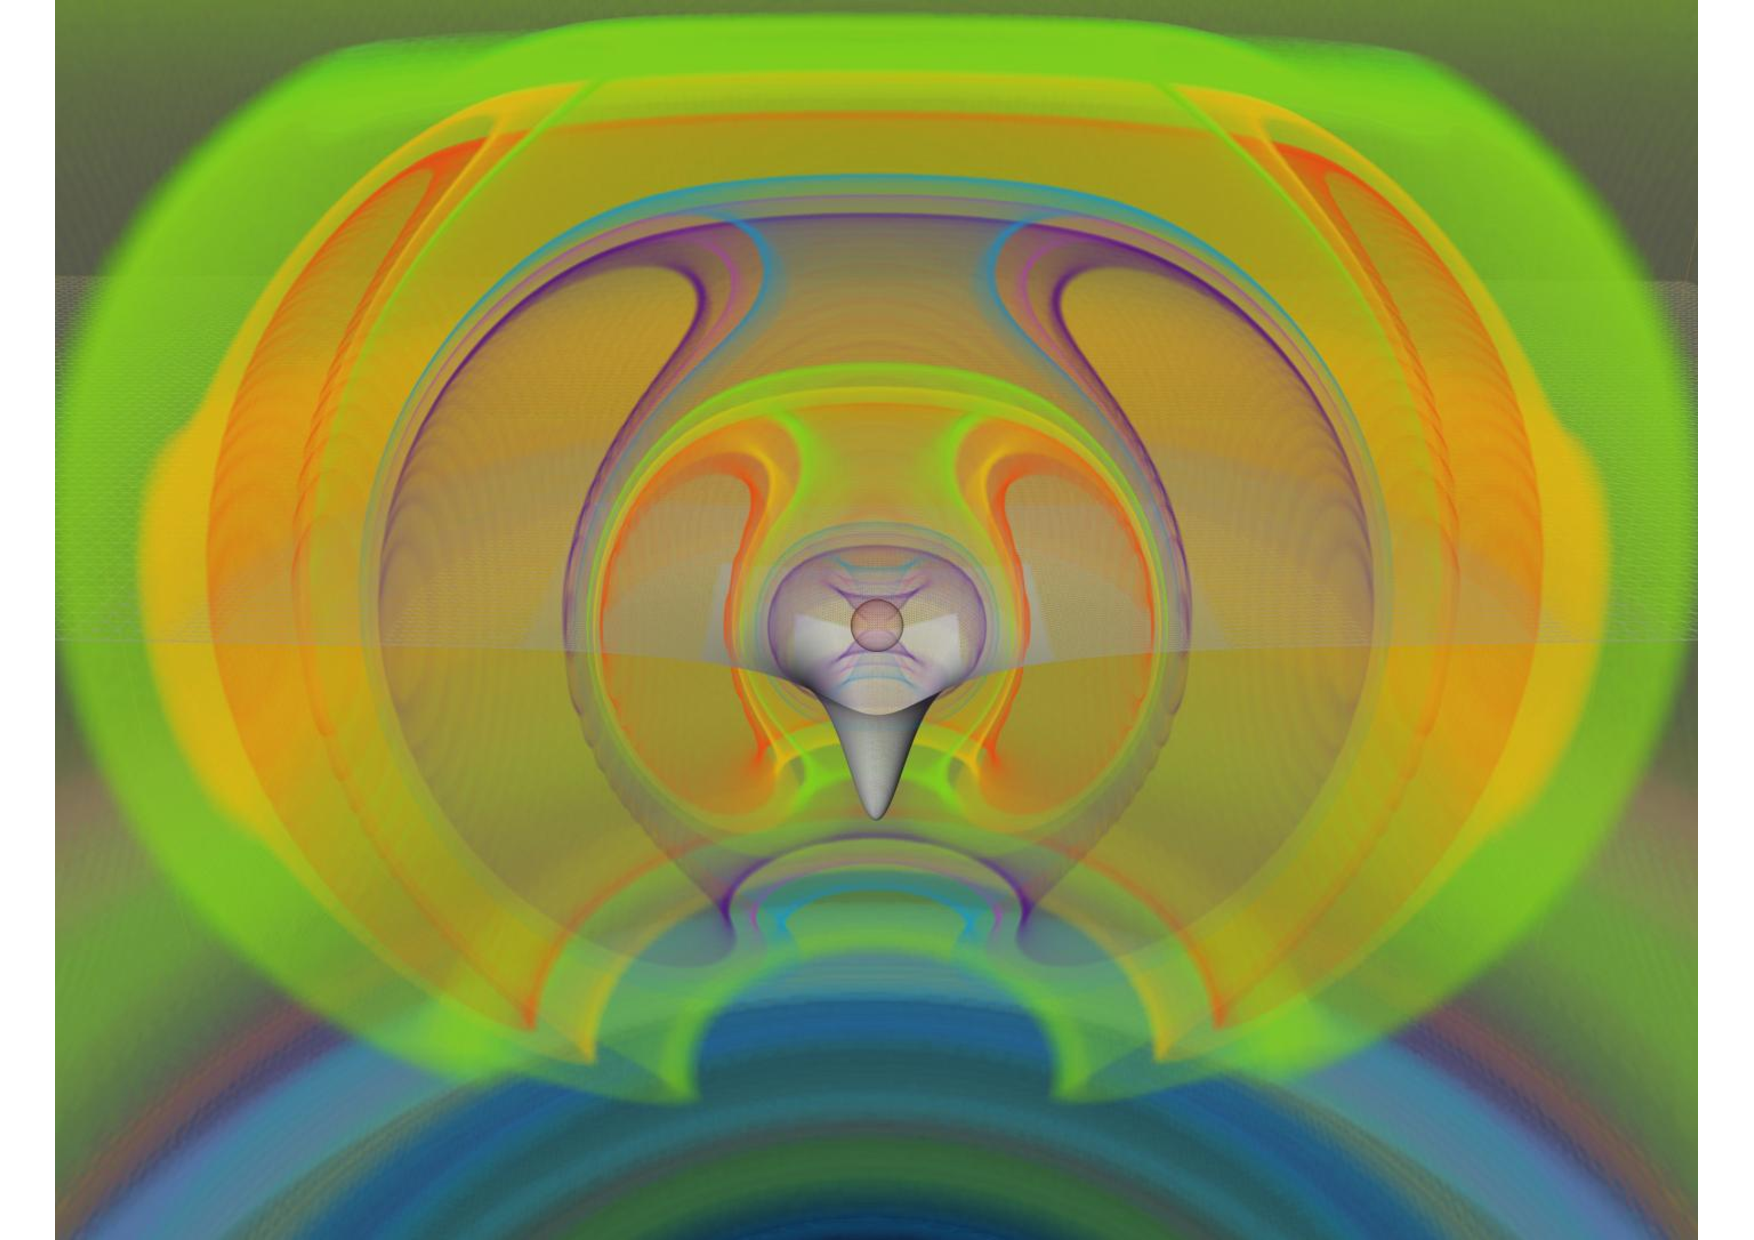
\includegraphics[width=0.88\linewidth,height=0.48\textheight,keepaspectratio]{../figs/pdf/en/fig-08-01.pdf}

% DOCX paragraph 1146
\caption{\emph{Simulación numérica de las ondas gravitatorias emitidas por un agujero negro perturbado. © R. Kaehler / LR.}}\label{fig:08-01}
\end{figure}

% DOCX paragraph 1148
En la figura \ref{fig:08-01} se muestra este tipo de ondas, resultado de una simulación numérica. La imagen detalla las ondas gravitatorias producidas en los primeros instantes en los que una estrella de neutrones casi esférica colapsa y se convierte en un agujero negro que aún no tiene una simetría esférica perfecta, sino pequeñas perturbaciones que van desapareciendo.\index{gravitatorio!colapso}

% DOCX paragraph 1149
Dejando de lado la simetría esférica\index{simetría esférica}, que es una excepción, ya que en la naturaleza es poco frecuente mantener una simetría esférica perfecta, hay que decir que, aunque sea fácil generar ondas gravitatorias, no todas las fuentes pueden producirlas con suficiente eficacia o a frecuencias que permitan detectarlas experimentalmente. Volveremos a estos dos aspectos, la eficacia de la emisión y la capacidad de detección, más adelante en este capítulo. Por el momento, concentrémonos en su efecto sobre el resto del espaciotiempo cuando se propagan.

% DOCX paragraph 1150
Para explicar qué sucede cuando interaccionamos con una onda gravitatoria, emplearé una analogía con un tipo de onda más cercano a nuestra experiencia cotidiana: las ondas generadas en la superficie perturbada de un lago. Imaginemos que nos encontramos sobre una colchoneta hinchable, flotando pacíficamente en la superficie de un lago perfectamente tranquilo, en un día soleado y sin viento. En un momento dado vemos a alguien saltar desde una barca en la distancia. Su impacto con el agua produce una perturbación que se extiende hacia fuera, con un frente esencialmente esférico y una amplitud decreciente, pues el frente de onda se distribuye por una superficie cada vez mayor. Cuando nos alcanza, la perturbación es muy pequeña, y su longitud de onda, la separación entre crestas sucesivas, será mucho mayor que el tamaño de nuestra colchoneta, que podemos considerar puntual, es decir, de tamaño despreciable. En una primera aproximación, o, en un lenguaje matemático más preciso, a primer orden en la perturbación, podemos decir que las ondas serán transversales, de modo que nuestra colchoneta comenzará a oscilar con un movimiento periódico en dirección vertical, perpendicular a la dirección de propagación de la onda. En este ejemplo, las ondas en el agua se encargan, en esencia, de transferir al resto del lago la energía cinética liberada por la persona que saltó de la barca. Una vez que haya pasado por completo el tren de ondas, es decir, la secuencia de ondas provocada por el salto, la colchoneta volverá a su posición inicial, en reposo, y nosotros podremos volver a relajarnos.\textsuperscript{\hyperlink{note:08-02}{2}}

% DOCX paragraph 1151
Por analogía con esta descripción, podemos llevar a cabo un experimento mental. Imaginemos que en algún lugar del universo se producen ondas gravitatorias, mediante procesos que describiremos más adelante, y que nos alcanzan en una dirección perpendicular a la superficie del lago, con una longitud de onda de nuevo mayor, aunque no mucho, que el tamaño de nuestra colchoneta. Como las ondas gravitatorias son transversales, la perturbación que propagan no se puede medir como una variación de la posición vertical de la colchoneta. Más bien, generan cambios locales en el valor de la curvatura. Dicho con más precisión, al cambiar la curvatura local, las ondas gravitatorias generarán «fuerzas de marea\index{ondas gravitatorias!fuerzas de marea}\index{fuerzas de marea}», que inducirán variaciones en la posición de objetos no sujetos a fuerzas externas. Es algo parecido a las fuerzas de marea que ejerce la Luna\index{Luna} sobre la Tierra y que ocasionan el desplazamiento de masas líquidas en nuestro planeta. Así pues, los campos de marea que nos alcanzarían en nuestro experimento mental inducirían deformaciones tanto en nosotros como, sobre todo, en el agua que nos rodea. Estas deformaciones son de un tipo muy específico, \emph{cuadrupolar}, y consisten en una «compresión» en una dirección dada y un «estiramiento» en la dirección perpendicular. Como veremos más adelante, estas variaciones serán periódicas y se emitirán a la misma frecuencia que las ondas, que puede ser constante o variar con el tiempo.

% DOCX paragraph 1152
Para entender mejor qué sentiríamos en nuestro experimento mental, podemos fijarnos en la figura \ref{fig:08-02}, que muestra las deformaciones\index{ondas gravitatorias!deformaciones} cuadrupolares que sufriría el \emph{Hombre de Vitruvio} de Leonardo da Vinci\index{Leonardo da Vinci} si lo atravesara una onda gravitatoria. Por fortuna, las ondas gravitatorias que llegan a la Tierra son tan débiles que no solo no producen deformaciones apreciables en nuestros cuerpos, sino que hay que construir dispositivos de gran sensibilidad para detectarlas.

% DOCX paragraph 1153
\begin{figure}[htbp]
\centering
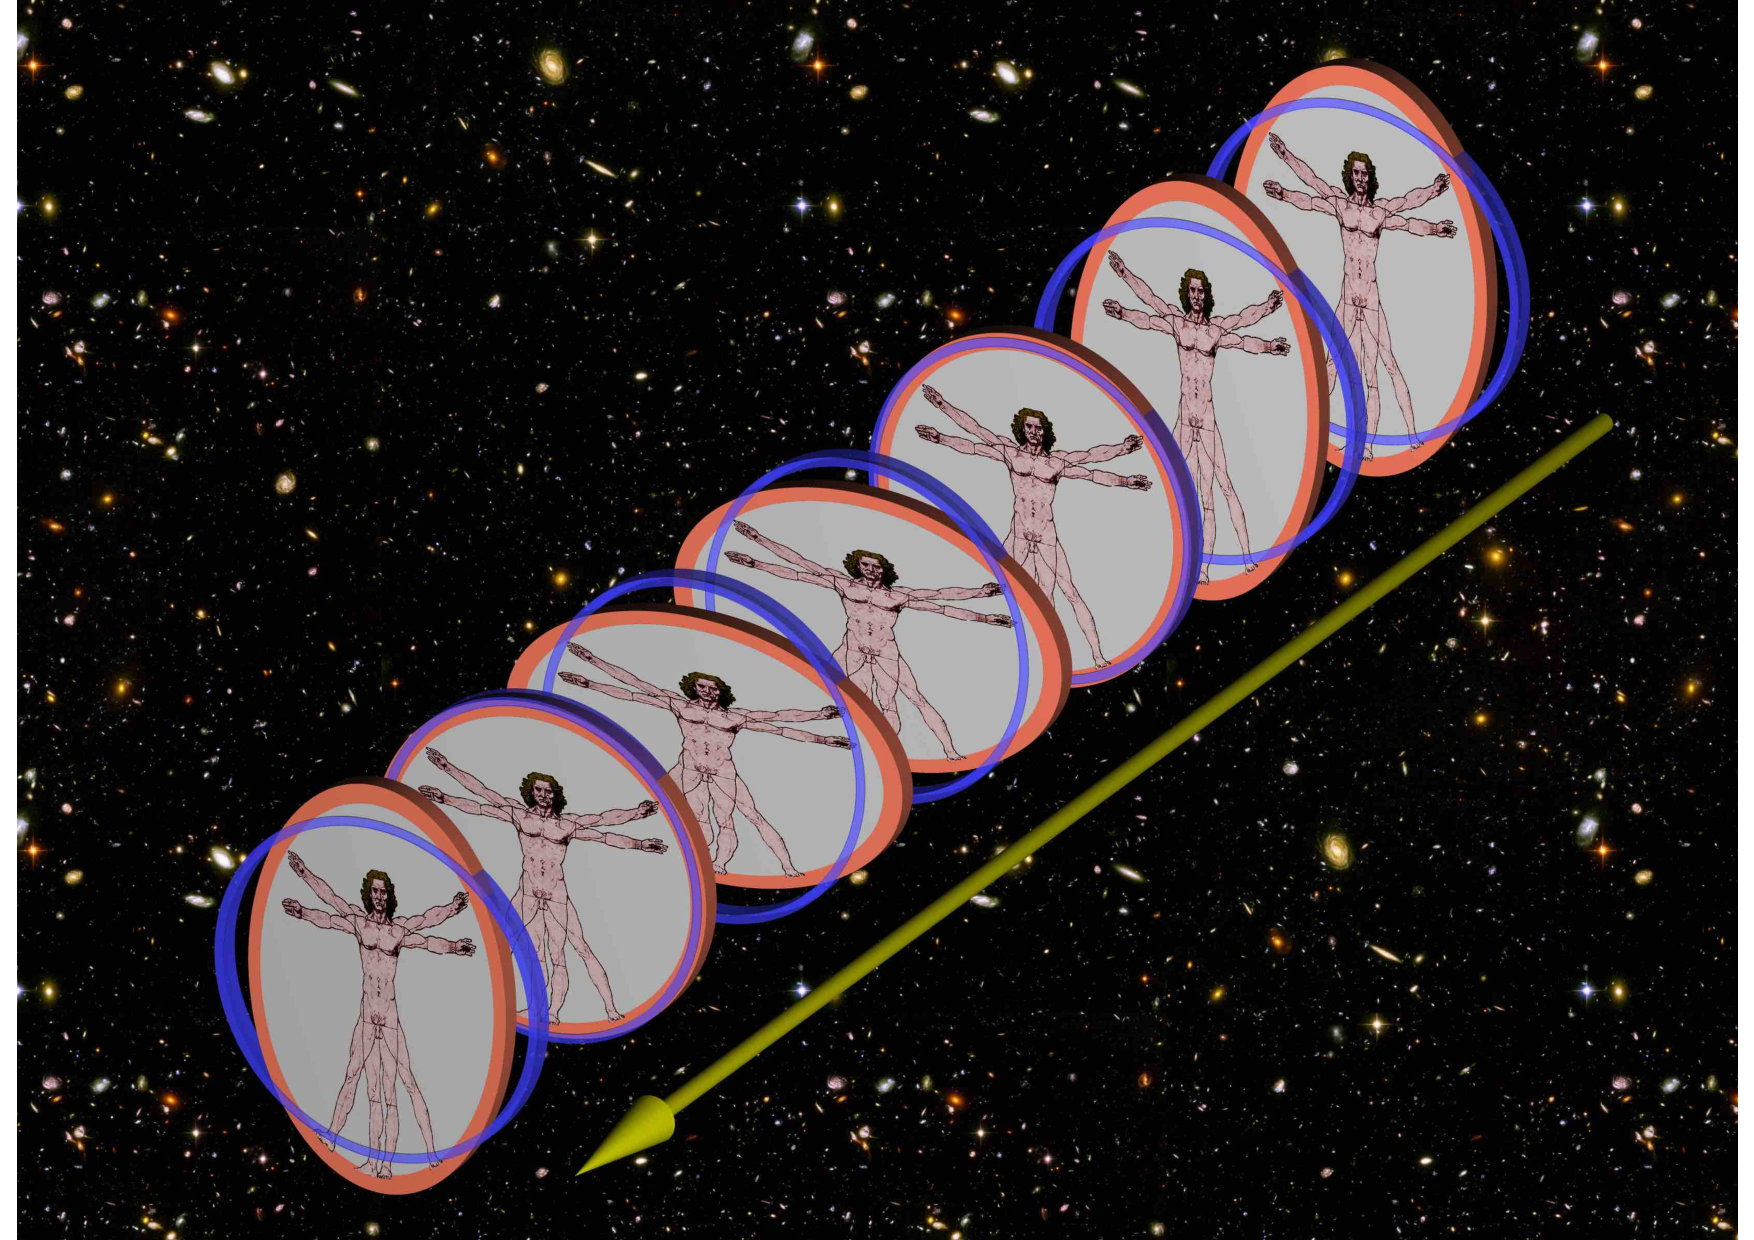
\includegraphics[width=0.88\linewidth,height=0.48\textheight,keepaspectratio]{../figs/pdf/en/fig-08-02.pdf}

% DOCX paragraph 1154
\caption{\emph{Deformación cuadrupolar del Hombre de Vitruvio\index{Leonardo da Vinci!Hombre de Vitruvio} al ser atravesado por una onda gravitatoria. © M. Pössel (AEI) / LR.}}\label{fig:08-02}
\end{figure}

% DOCX paragraph 1155
Es importante comentar aquí un aspecto al que no siempre se le da la relevancia que merece. En su formulación matemática, las ecuaciones de Einstein solo se comportan como ondas si se dan unas condiciones precisas: un espaciotiempo\index{espaciotiempo!plano} vacío\index{vacío}, un campo débil y planitud asintótica. Estas condiciones, por supuesto, no se dan en las proximidades de la fuente, donde el espaciotiempo tiene una curvatura acusada y muy dinámica. Sin embargo, sí se cumplen donde estamos nosotros, a una gran distancia de las fuentes, donde estas perturbaciones se comportan como ondas. Para nosotros, como observadores lejanos, las perturbaciones de la curvatura se comportarán por tanto como ondas de dos tipos, o con dos grados de \emph{polarización\index{polarización} lineal\index{polarización!lineal (más)}\index{polarización!lineal (cruz)}}. Uno se denomina \emph{polarización «más»}, indicada con el símbolo +, y el otro, idéntico pero girado 45 grados, \emph{polarización «cruz»}, indicada con el símbolo ×. Para hacernos una idea concreta de la diferencia entre las dos polarizaciones, podemos referirnos de nuevo a la figura \ref{fig:08-02}, que muestra los efectos de la polarización «más». En cambio, la polarización «cruz» no comprimiría ni estiraría al \emph{Hombre de Vitruvio\index{Leonardo da Vinci!Hombre de Vitruvio}} en la dirección entre la cabeza y los pies, sino en una dirección diagonal a esta.\textsuperscript{\hyperlink{note:08-03}{3}}

% DOCX paragraph 1156
En general, el grado de polarización\index{ondas gravitatorias!polarización (véase polarización)} de las ondas gravitatorias refleja las propiedades de la fuente. Las fuentes astrofísicas realistas producirán radiación\index{gravitatorio!radiación} que contiene una mezcla de estas polarizaciones, aunque es posible generar radiación gravitatoria en una sola polarización si se dan ciertas condiciones especiales. Conocidas estas propiedades, centrémonos ahora en por qué es importante estudiar las ondas gravitatorias.

% DOCX paragraph 1159
\section{Ondas gravitatorias y electromagnéticas}\label{sec:08-comparison}

% DOCX paragraph 1161
A menudo se señala que la detección combinada de ondas electromagnéticas y gravitatorias ha marcado el nacimiento de la \emph{astronomía multimensajero\index{astronomía!multimensajero (ondas gravitatorias)} de ondas gravitatorias}, abriendo una nueva «ventana» al universo. Ambas afirmaciones son correctas, aunque tal vez un poco oscuras.

% DOCX paragraph 1162
Veamos qué significan y comencemos por aclarar el sentido de astronomía «multimensajero\index{astronomía!multimensajero}\index{astronomía!multimensajero (ondas gravitatorias)}». La definición formal dice que se trata de una rama de la astronomía en la cual el conocimiento científico se alcanza a través de distintos canales de información, llamados «mensajeros». Concretamente, además del evidente canal electromagnético, es decir, la luz emitida por los objetos celestes en las distintas bandas, la astronomía multimensajero\index{astronomía multimensajero} recurre a otros mensajeros, como los neutrino\index{neutrino}s, por ejemplo los emitidos en las explosiones de supernova, o las ondas gravitatorias. En este último caso también se denomina \emph{astronomía multimensajero de ondas gravitatorias}. Su importancia reside en que, al usar más de un canal para obtener información, y dado que la información contenida en los diversos canales puede diferir sustancialmente, tiene el potencial de ser mucho más «rica» que la astronomía tradicional.

% DOCX paragraph 1163
Para ilustrar mejor lo que quiero decir, me permitirán que ofrezca un ejemplo que en mi opinión encaja muy bien y es fácil de entender. Imagínese el lector que participa en uno de los muchos y hermosos festivales característicos del verano en Italia, y que el programa incluye fuegos artificiales a última hora de la noche. Como le apasionan los fuegos artificiales, ha elegido con mucho cuidado el mejor lugar para disfrutar del espectáculo. Un lugar que ofrece una excelente perspectiva elevada, lo bastante lejano para abarcar toda la función con la vista, pero lo bastante cercano para disfrutar plenamente del estruendo de las explosiones. En esencia, imaginemos que estamos bebiendo una copa de vino, inmersos en la calidez de la noche de verano y disfrutando de unos fuegos artificiales inolvidables.

% DOCX paragraph 1164
Ahora pensemos en cómo sería esta experiencia si nos viéramos privados de la vista o del oído. Si no pudiéramos distinguir las luces de los fuegos, percibiríamos toda la función como una secuencia de explosiones, unas intensas y graves, otras más débiles y agudas, que apenas transmitirían su espectacularidad. Si, en cambio, no pudiéramos oír el sonido de la pirotecnia, estaríamos ante una secuencia de imágenes coloridas y tal vez fascinantes, pero poco emocionantes, como si todo estuviera ocurriendo en otro planeta. En varias ocasiones he observado por casualidad fuegos artificiales desde un avión que volaba bajo, y puedo asegurar que es mucho menos emocionante.

% DOCX paragraph 1165
Este ejemplo ilustra que los fuegos artificiales pueden considerarse, a efectos prácticos, un fenómeno \emph{multimensajero}. La razón es que su información nos llega tanto por las ondas sonoras, el primer mensajero, como por las ondas electromagnéticas, el segundo. Gracias a esta analogía se puede apreciar de forma plena y directa cuánto más ricas e informativas pueden ser las observaciones astronómicas multimensajero en comparación con las tradicionales. Nos permiten investigar diferentes aspectos de una fuente porque los transmiten distintos mensajeros.

% DOCX paragraph 1166
Si nos centramos en cómo difieren las ondas gravitatorias de otros mensajeros, nos será más fácil apreciar que representan un tipo de mensajero muy distinto. La gran mayoría de la información que recibimos sobre nuestro universo nos llega a través de las ondas electromagnéticas. Cubren un espectro\index{espectro!electromagnético} muy amplio, desde la banda de radio hasta la de rayos gamma, pero tienen una propiedad en común: revelan detalles sobre el estado \emph{termodinámico} de las fuentes, a saber, su densidad y temperatura. Al mismo tiempo, los componentes de la luz, los fotones, interaccionan con la materia que encuentran de camino hacia nosotros, y experimentan absorción o emisión adicional. De hecho, una fuente astronómica puede quedar eclipsada, parcial o totalmente, por el material interpuesto entre nosotros y ella. Las ondas gravitatorias son algo diferentes porque transmiten un campo gravitatorio de marea, de modo que solo están débilmente acopladas a las fuerzas que mantienen unidos los objetos astronómicos. Como resultado, se propagan casi sin perturbaciones y nos proporcionan información sobre los movimientos globales de las fuentes a frecuencias muy distintas de las de las ondas electromagnéticas. La información que transmiten es, por tanto, necesariamente diferente y complementaria.\index{estado termodinámico}

% DOCX paragraph 1167
La tabla siguiente resume las diferencias, a veces radicales, entre las ondas electromagnéticas\index{ondas gravitatorias!ondas electromagnéticas (frente a)} (EM) y las ondas gravitatorias\index{ondas electromagnéticas!ondas gravitatorias (frente a)} (OG), y entre los tipos de información que transmiten.

% DOCX paragraph 1168
{\small
\setlength{\tabcolsep}{5pt}
\begin{longtable}{@{}>{\raggedright\arraybackslash}p{0.48\linewidth}>{\raggedright\arraybackslash}p{0.48\linewidth}@{}}
\toprule
% DOCX table after paragraph 1168, row 0, column 0
\textbf{Ondas electromagnéticas}
&
% DOCX table after paragraph 1168, row 0, column 1
\textbf{Ondas gravitatorias}
\\[6pt]
\midrule
% DOCX table after paragraph 1168, row 1, column 0
Son oscilaciones de los campos eléctrico y magnético que se propagan por el espaciotiempo.
&
% DOCX table after paragraph 1168, row 1, column 1
Son oscilaciones del propio espaciotiempo.
\\[6pt]
% DOCX table after paragraph 1168, row 2, column 0
Las más simples corresponden a la radiación\index{dipolo!radiación} dipolar, generada por un dipolo\index{dipolo!eléctrico} oscilante: dos cargas eléctricas opuestas.
&
% DOCX table after paragraph 1168, row 2, column 1
Las más simples corresponden a la radiación\index{cuadrupolo!radiación} cuadrupolar, generada por un cuadrupolo de masa\index{cuadrupolo!masa} oscilante: una distribución no circular de masa.
\\[6pt]
% DOCX table after paragraph 1168, row 3, column 0
Son casi siempre el resultado de la superposición incoherente de contribuciones de millones de electrones, átomos o moléculas.
&
% DOCX table after paragraph 1168, row 3, column 1
Se producen por el movimiento coherente de grandes cantidades de masa y energía, ya sea en forma de objetos astronómicos o de concentraciones de energía.
\\[6pt]
% DOCX table after paragraph 1168, row 4, column 0
Nos muestran los detalles del estado termodinámico\index{estado termodinámico}, temperatura y densidad, de las fuentes que las producen.
&
% DOCX table after paragraph 1168, row 4, column 1
Nos muestran los detalles de la dinámica y las propiedades globales, tamaño, masa y velocidad, de grandes concentraciones de masa-energía.
\\[6pt]
% DOCX table after paragraph 1168, row 5, column 0
Sus longitudes de onda son muy cortas en comparación con el tamaño de las fuentes astronómicas. Por tanto, es posible obtener «imágenes» de las fuentes.
&
% DOCX table after paragraph 1168, row 5, column 1
Sus longitudes de onda suelen ser comparables al tamaño de las fuentes que las producen, o incluso mayores. Por tanto, no es posible obtener «imágenes» de las fuentes.
\\[6pt]
% DOCX table after paragraph 1168, row 6, column 0
Sufren absorción, difusión y dispersión por la materia que encuentran en su camino.
&
% DOCX table after paragraph 1168, row 6, column 1
Se propagan sin perturbaciones, a la velocidad de la luz, a través de todo tipo de materiales.
\\[6pt]
% DOCX table after paragraph 1168, row 7, column 0
Las emitidas por objetos celestes tienen un espectro\index{espectro!electromagnético} esencialmente independiente de la masa de la fuente; por ejemplo, las emisiones de agujeros negros estelares y supermasivos son muy parecidas.
&
% DOCX table after paragraph 1168, row 7, column 1
Las emitidas por objetos celestes tienen un espectro que depende de la masa de la fuente: la frecuencia de las ondas gravitatorias\index{espectro!ondas gravitatorias} de agujeros negros estelares es mucho mayor que la de las procedentes de agujeros negros supermasivos.
\\[6pt]
% DOCX table after paragraph 1168, row 8, column 0
Sus longitudes de onda son menores que los radios de curvatura de los objetos que encuentran al propagarse. Por eso experimentan el efecto de lente gravitatoria\index{gravitatorio!efecto de lente}, es decir, distorsión y amplificación.
&
% DOCX table after paragraph 1168, row 8, column 1
Sus longitudes de onda son comparables o superiores a los radios de curvatura de los objetos que encuentran al propagarse. Por eso el efecto de lente gravitatoria es menos pronunciado y más difícil de medir.
\\[6pt]
\bottomrule
\end{longtable}
}


% DOCX paragraph 1170
Tras esta breve comparación, creo que queda claro que la posibilidad de observar un mismo fenómeno astrofísico a través de su emisión de ondas gravitatorias y electromagnéticas representa una oportunidad fantástica para multiplicar y ampliar la información recogida. El primer suceso de ondas gravitatorias detectado fue GW150914\index{GW150914}, cuyo nombre indica que se trata de un suceso de ondas gravitatorias (GW, por sus siglas en inglés) detectado el 14 de septiembre de 2015. La señal la produjo un sistema binario de agujeros negros y, durante los meses posteriores a su detección, los astrónomos buscaron una «contrapartida electromagnética\index{contrapartida electromagnética}», es decir, rastros de una emisión electromagnética correspondiente en todas las bandas posibles, desde los rayos gamma hasta la radio. Por desgracia, no se identificó ninguna contrapartida electromagnética\index{contrapartida electromagnética}, y sigue sin haberse encontrado, varios años después. Tampoco se ha conseguido detectar una contrapartida electromagnética de otras señales de ondas gravitatorias procedentes de sistemas binarios de agujeros negros, de las que actualmente hay más de 60. Por fortuna, esta situación bastante frustrante cambió en 2017 con el suceso GW170817\index{GW170817}: la fusión de un sistema binario de estrellas de neutrones que nos regaló una fantástica exhibición de fuegos artificiales cósmicos. Hablaremos de él dentro de poco.

% DOCX paragraph 1173
\section{¿Cómo detectamos las ondas gravitatorias?}\label{sec:08-detectors}

% DOCX paragraph 1175
Hemos visto que la producción de ondas gravitatorias no es en absoluto un fenómeno raro o complejo; todo lo contrario. Lo que las hace tan inusuales en nuestra experiencia es que la amplitud de las ondas gravitatorias que recibimos habitualmente en la Tierra no es lo bastante grande para medirla con un dispositivo experimental. Para entender por qué, debemos recordar primero que la propagación de una onda gravitatoria se manifiesta a través de campos de marea que inducen una variación del tamaño de los objetos que encuentran. Dentro de poco hablaremos con más detalle de qué produce ondas gravitatorias con una amplitud que nos permita detectarlas, pero puedo adelantar que, incluso considerando las fuentes astrofísicas más intensas que cabe imaginar, un sistema binario de agujeros negros, y teniendo en cuenta las distancias típicas de estas fuentes, la amplitud «\emph{h}» con la que nos llegan sus ondas gravitatorias es de tan solo \emph{h} \(\simeq \ \)10\textsuperscript{--21}, un número tan pequeño que equivale a una parte en 1\,000\,000\,000\,000\,000\,000\,000. Es difícil imaginar la precisión necesaria para medir un número tan pequeño, pero sería como medir una longitud igual a una milmillonésima del diámetro de un átomo o, de manera equivalente, la distancia entre la Tierra y Próxima Centauri\index{Proxima Centauri@Próxima Centauri} ¡con una precisión de 40 micras!

% DOCX paragraph 1176
Tal precisión parecería imposible de alcanzar en la práctica. Y, sin embargo, después de décadas de investigación y mejoras continuas, los modernos detectores de ondas gravitatorias, como LIGO\index{LIGO} o Virgo\index{Virgo}, ya pueden operar con esa precisión. Así pues, ¿cómo consiguen semejantes resultados?

% DOCX paragraph 1177
La respuesta está en una técnica de la que hablamos en el capítulo anterior: la interferometría. En el caso de los detectores\index{ondas gravitatorias!detectores} de ondas gravitatorias, el funcionamiento básico implica un dispositivo relativamente sencillo, basado en un experimento que realizaron a finales del siglo XIX los físicos estadounidenses Albert\index{Michelson!Albert} Michelson y Edward\index{Morley!Edward} Morley para medir el movimiento de la Tierra a través de un medio hipotético, el «éter\index{eter@éter}». Por desgracia, el experimento mostró que ese medio no existe. Sin embargo, quedó el ingenioso dispositivo experimental, conocido como \emph{interferómetro\index{Michelson!interferómetro}\index{Morley!interferómetro} de Michelson-Morley\index{interferómetro!Michelson-Morley}}, que más tarde se adoptó para detectar ondas gravitatorias.

% DOCX paragraph 1178
La figura \ref{fig:08-03} muestra un esquema simplificado de este interferómetro\index{interferómetro}. Como se puede ver, una fuente de luz lo más coherente y estable posible produce un haz luminoso. Hoy se emplean láseres potentes, pero a finales del siglo XIX la tecnología era más rudimentaria. Un espejo semirreflectante\index{espejo!semirreflectante} recoge ese haz. Estos espejos\index{detector de ondas gravitatorias!espejos} reflejan solo una parte de la luz incidente y dejan pasar otra, como los que se usan en las comisarías para observar una sala de interrogatorios sin ser vistos. En los interferómetros de ondas gravitatorias se emplean espejos muy sofisticados que reflejan exactamente el 50 por ciento de la luz y dejan pasar el 50 por ciento restante. Supongamos, además, que el espejo está colocado a 45 grados respecto al haz incidente, como muestra la figura. En ese caso, «divide» el haz en dos; de hecho, estos espejos también se llaman «divisores de haz». La luz se propaga en dos direcciones perpendiculares, que representan los llamados «\emph{brazos}» del interferómetro. Los brazos se pueden alargar virtualmente añadiendo otro espejo y creando lo que se llama una cavidad de Fabry-Pérot.\index{detector de ondas gravitatorias!divisor de haz}

% DOCX paragraph 1180
\begin{figure}[htbp]
\centering
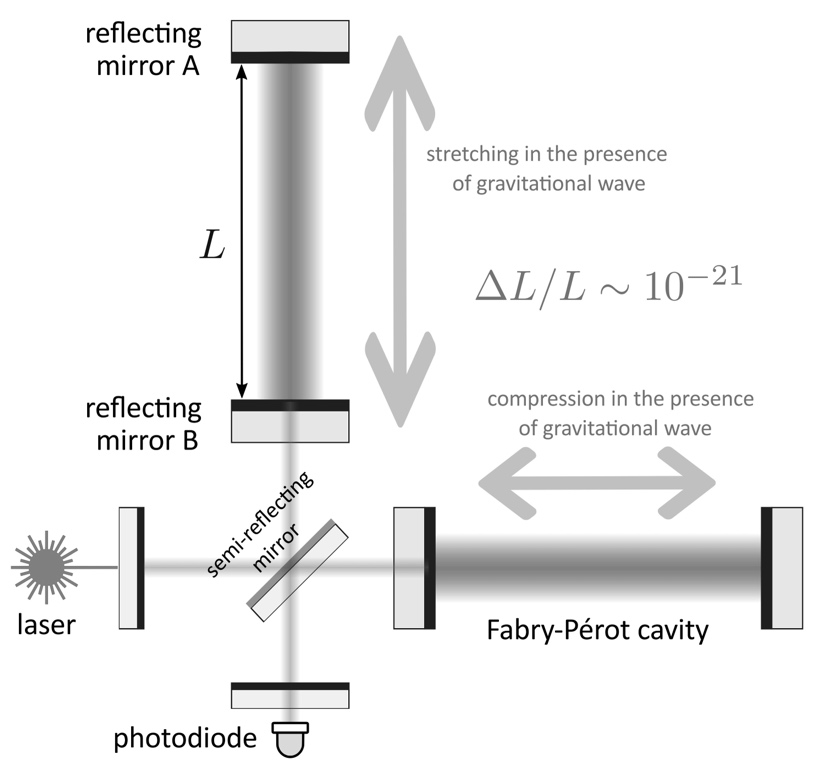
\includegraphics[width=0.88\linewidth,height=0.48\textheight,keepaspectratio]{../figs/source/en/fig-08-03.jpeg}

% DOCX paragraph 1182
\caption{\emph{Representación esquemática de un detector interferométrico de ondas gravitatorias.}}\label{fig:08-03}
\end{figure}

% DOCX paragraph 1184
En el experimento original de 1887, la longitud de los dos brazos era de unos diez metros, decididamente insuficiente para medir ondas gravitatorias. Como la variación relativa de los brazos inducida por una onda gravitatoria, normalmente indicada como \emph{ΔL/L}, es igual a la amplitud de la propia onda, que hemos visto que es \emph{h} ≃ 10\textsuperscript{--21}, la tecnología actual solo permite medirla si la longitud de los brazos del interferómetro, \emph{L}, es de unos pocos kilómetros. Por esta razón, los detectores interferométricos LIGO\index{detector de ondas gravitatorias!LIGO}, uno situado en Livingston, Luisiana, y el otro en Hanford, en el estado de Washington, tienen brazos de cuatro kilómetros. El detector Virgo\index{Virgo}\index{detector de ondas gravitatorias!Virgo}, en Cascina, cerca de Pisa, tiene brazos algo más cortos, de tres kilómetros.

% DOCX paragraph 1185
El divisor de haz divide el haz láser inicial en dos haces perpendiculares que recorren los brazos hasta llegar al primer espejo reflector\index{espejo!reflector}, suspendido de finos hilos de silicio, el «espejo A» del brazo vertical, que refleja los haces incidentes. Como cabe imaginar, estos espejos son más elaborados que los habituales; de hecho, son pequeñas maravillas tecnológicas. Además de tener casi veinte centímetros de espesor y pesar varias decenas de kilos, su superficie es tan lisa que la rugosidad es del orden de un nanómetro, es decir, unas pocas milmillonésimas de metro. Por otro lado, mientras que los espejos de nuestras casas tienen una reflectividad de entre el 80 y el 90 por ciento, la de estos supera el 99,9999 por ciento. En otras palabras, solo se absorbe, en lugar de reflejarse, un fotón\index{foton@fotón} de cada millón.

% DOCX paragraph 1186
Una vez reflejados por estos instrumentos asombrosos, los haces láser regresan, se reúnen, atraviesan de nuevo el divisor de haz e interfieren en un dispositivo electrónico muy sensible a la luz llamado «\emph{fotodiodo\index{detector de ondas gravitatorias!fotodiodo}}». En general, en ausencia de radiación\index{gravitatorio!radiación} gravitatoria\index{radiación!gravitatoria}, el interferómetro puede «ajustarse» para que, al regresar al divisor, los dos haces estén perfectamente «\emph{en fase}» o «\emph{en oposición de fase}». De este modo producen interferencia\index{interferencia} constructiva cuando están en fase, pues su luz se suma, o destructiva cuando están en oposición de fase, pues su luz se cancela. A efectos prácticos, conviene que la interferencia medida por el fotodiodo sea destructiva y, de hecho, todo el interferómetro se ajusta para que el fotodiodo se encuentre en la «franja oscura».

% DOCX paragraph 1187
El paso de una onda gravitatoria que se propagase en una dirección perpendicular al plano de los dos brazos produciría una distorsión de marea y, por tanto, una variación relativa de la longitud de los brazos. Esto, a su vez, produciría un desfase entre los trayectos que recorre la luz en ambos brazos y, en consecuencia, una variación de la interferencia\index{interferencia} en el fotodiodo, que ya no estaría sincronizado en una franja oscura. Cuanto mayor fuera la amplitud de la onda gravitatoria, mayor sería la distorsión de los brazos y, por tanto, el desfase de la luz recombinada en el fotodiodo.

% DOCX paragraph 1188
Acabo de describir, pasando alegremente por alto algunos detalles importantes, el funcionamiento básico de un experimento interferométrico clásico de Michelson-Morley. Sin embargo, aunque consiguiéramos construir un interferómetro de este tipo, con brazos de cuatro kilómetros, ¡no detectaríamos ninguna onda gravitatoria! Esto se debe a que las deformaciones que producen, y por tanto la amplitud de nuestra \emph{señal}, seguirían siendo demasiado pequeñas en comparación con las que inevitablemente produce el entorno, que representan el llamado \emph{ruido\index{ruido}}. Como no podemos cambiar la amplitud de la señal, determinada única y exclusivamente por las propiedades de la fuente, nuestra única esperanza de detectarla consiste en reducir el ruido todo lo posible. Para ello hay que recurrir a una serie de medidas experimentales destinadas a reducir el nivel de ruido por debajo del de la señal, es decir, a aumentar la relación señal-ruido\index{relación señal-ruido}\index{ruido!relación señal-ruido}. Es algo parecido a estar en una habitación y oír una melodía que nos resulta familiar pero no conseguimos identificar porque el ruido de las otras personas nos impide distinguir claramente las notas. Si no podemos subir el volumen de la música, la única opción es reducir el ruido, así que pedimos a los demás que guarden silencio un momento.

% DOCX paragraph 1189
Durante los últimos 40 años se han desarrollado numerosas técnicas para reducir las distintas fuentes de ruido que afectan a los modernos detectores de ondas gravitatorias. Por interesantes e ingeniosas que sean, explicarlas exigiría más tiempo del que nos queda en esta última parte del viaje. Lo que importa aquí es subrayar que detectores como LIGO y Virgo representan el resultado del trabajo conjunto de miles de personas y que, al igual que los radiotelescopios de la colaboración EHT\index{radiotelescopio!EHT} o los aceleradores del CERN\index{CERN}, deben verse como la máxima expresión de la capacidad tecnológica humana. En definitiva, estos detectores representan la única herramienta disponible para detectar las fuentes de ondas gravitatorias de las que hablaremos en la siguiente sección.

% DOCX paragraph 1192
\section{¿Quién produce las ondas?}\label{sec:08-sources}

% DOCX paragraph 1194
El título de esta sección está incompleto a propósito. A estas alturas sabemos que cualquier variación no esférica en el tiempo de una concentración de masa\index{masa!equivalencia con la energía}-energía\index{energia@energía!equivalencia con la masa} produce ondas gravitatorias. Por tanto, el título completo, aunque evidentemente demasiado largo, debería haber sido: «¿Cuáles son las fuentes\index{ondas gravitatorias!fuentes} de ondas gravitatorias que podemos detectar?». La respuesta es bastante sencilla: todas las fuentes lo bastante «potentes», es decir, capaces de liberar cantidades de energía suficientemente grandes en forma de ondas gravitatorias.

% DOCX paragraph 1195
Hace ya bastante tiempo que no propongo una ecuación, y desde luego no quiero que los lectores pierdan la costumbre de leerlas\ldots{} Por eso ofrezco a continuación una expresión aproximada, pero compacta, de la luminosidad, es decir, la cantidad de energía por unidad de tiempo, de una fuente de ondas gravitatorias\index{luminosidad!ondas gravitatorias}. Esta famosa expresión, conocida también como «\emph{fórmula\index{cuadrupolo!fórmula} del cuadrupolo}», nos dice que la luminosidad de una fuente de ondas gravitatorias viene dada simplemente por las siguientes propiedades básicas de la fuente; advierto que omito deliberadamente cualquier factor numérico:

% DOCX paragraph 1197
\begin{equation}\label{eq:08-01}
L_{GW} \simeq \textcolor{gray}{Gc}\left( \frac{M}{R} \right)^{2}\left( \frac{v}{v} \right)^{6} \simeq \textcolor{gray}{\frac{c^{5}}{G}}\left( \frac{r_{s}}{R} \right)^{2}\left( \frac{v}{v} \right)^{6}
\end{equation}

% DOCX paragraph 1199
En la fórmula, \emph{M} es la masa de la fuente, \emph{R} su tamaño característico, por ejemplo el radio si pensamos en una estrella o un agujero negro, y \emph{v} la velocidad media a la que se mueve. Como siempre, he dejado en gris las partes relacionadas con constantes, que no desempeñan un papel importante a la hora de entender la ecuación.

% DOCX paragraph 1200
Si miramos con un poco más de atención la ecuación \eqref{eq:08-01}, vemos que contiene tres términos: el primero, a la izquierda, es simplemente la definición de luminosidad; el segundo, en el centro, expresa la luminosidad en función de la masa y la velocidad; el último, a la derecha, utiliza una magnitud que vimos en el capítulo 6, el radio de Schwarzschild: \emph{r\textsubscript{s}=2GM/c\textsuperscript{2 }}(recuérdese la ecuación (6.1)). Centrémonos primero en la parte central de la fórmula \eqref{eq:08-01}. Nos dice que la luminosidad es proporcional a una magnitud con la que nos hemos encontrado varias veces durante nuestro viaje, la compacidad de la fuente, \emph{M/R}, y, en particular, a su cuadrado. Además, la luminosidad también es proporcional a la velocidad de la fuente, expresada en unidades de la velocidad de la luz, y, en particular, a su sexta potencia.

% DOCX paragraph 1201
En su sencillez, la ecuación \eqref{eq:08-01} aclara muchos detalles que quizá seguían oscuros hasta ahora. Como la mayoría de las estructuras astrofísicas tienen una compacidad muy pequeña y se mueven a velocidades muy inferiores a la de la luz, su luminosidad en ondas gravitatorias es inevitablemente diminuta. Tomemos el ejemplo concreto del Sol\index{compacidad!Sol}\index{luminosidad!Sol}. Hemos visto que su compacidad es del orden de \emph{M/R} ≃ 10\textsuperscript{--6}, como recuerda la ecuación (4.3), y que se desplaza por nuestra galaxia a unos 800\,000 kilómetros por hora, unas pocas milésimas de la velocidad de la luz. Por tanto, podemos usar la ecuación \eqref{eq:08-01} para calcular su luminosidad en ondas gravitatorias y obtener: \emph{L\textsubscript{GW}} ≃ 10\textsuperscript{8} vatios ≃ 10\textsuperscript{--18} \emph{L\textsubscript{EM}}. En otras palabras, la «luminosidad» del Sol en ondas gravitatorias es inferior a una milmillonésima de una milmillonésima de la que emite en forma de radiación electromagnética\index{radiación!electromagnética}. Y si esto es cierto para nuestra estrella, que aun así se mueve a una velocidad considerable y tiene cierta compacidad, resulta fácil imaginar lo inútil que sería tratar de generar ondas gravitatorias detectables aquí en la Tierra. Por ejemplo, imaginemos que queremos construir una fuente de ondas gravitatorias usando una masa de una tonelada, 1000 kilogramos, con un tamaño de un metro, que se mueva a cien kilómetros por hora. Podría ser un coche pequeño, pero pesado, que recorriera un circuito circular cerrado de un kilómetro de radio. En este caso, la amplitud de las ondas gravitatorias producidas sería tan pequeña como \emph{h} ≃ 10\textsuperscript{--43}: unas pocas millonésimas de una milmillonésima de una milmillonésima de lo que hoy pueden medir los mejores detectores. No creo que merezca la pena intentarlo\ldots{}

% DOCX paragraph 1202
Centrémonos ahora en la tercera parte de la ecuación \eqref{eq:08-01}. Nos dice que la luminosidad en ondas gravitatorias\index{luminosidad!ondas gravitatorias} es máxima cuando un objeto tiene dimensiones comparables a su radio de Schwarzschild y se mueve a una velocidad muy próxima a la de la luz. Tiene todo el sentido y explica por qué la primera señal de ondas gravitatorias que se midió procedía de un sistema binario de agujeros negros: son, sencillamente, las fuentes más potentes que cabe imaginar. Por definición, los componentes del sistema tienen un tamaño \emph{exactamente} igual al radio de Schwarzschild y se mueven a unos 2/3 de la velocidad de la luz en las etapas finales de sus órbitas de aproximación en espiral\index{orbita@órbita!aproximación en espiral}. Además, como forman parte de un sistema binario, ofrecen la máxima desviación posible de la simetría esférica\index{simetría esférica}.

% DOCX paragraph 1203
En resumen, la ecuación \eqref{eq:08-01} nos transmite un mensaje muy claro: si queremos tener alguna esperanza de detectar ondas gravitatorias con los detectores interferométricos actuales, debemos recoger la señal de objetos extremadamente compactos, es decir, con \emph{M}≃\emph{R}, de dimensiones comparables al radio de Schwarzschild, con \emph{R}≃\emph{r\textsubscript{S}}, y que se muevan a una velocidad próxima a la de la luz, con \emph{v}≃\emph{c}. Las ondas gravitatorias emitidas por fuentes de este tipo, situadas a unos pocos cientos de megapársecs, llegarán a la Tierra con una amplitud \emph{h}≃10\textsuperscript{--21} que, aunque esté en el límite de sensibilidad de nuestros instrumentos, en principio se puede medir.

% DOCX paragraph 1206
\section{La zoología de las fuentes de ondas gravitatorias}\label{sec:08-zoology}

% DOCX paragraph 1208
Ahora que sabemos qué hace falta para producir emisiones intensas de ondas\index{ondas gravitatorias!ondas} gravitatorias, resulta útil clasificar las diversas señales que podríamos detectar según las fuentes que las producen. Como veremos, las distintas fuentes imprimirán sus propiedades específicas en las características de las señales, que variarán en amplitud, frecuencia y duración.

% DOCX paragraph 1210
\emph{Señales impulsivas.} Son señales muy cortas, del orden de decenas de milisegundos o menos, que pueden producir distintas fuentes. Por ejemplo, se espera que aparezcan en asociación con explosiones de supernova\index{supernova} o con el colapso gravitatorio que da lugar a una estrella de neutrones, como ocurre con las supernovas, o a un agujero negro. Como son señales breves y evanescentes, sus «propiedades espectrales», la ventana de frecuencias en la que aparece la señal y su amplitud a las distintas frecuencias, no están bien definidas. Sin embargo, en general se trata de señales a frecuencias altas o muy altas, desde unos pocos cientos de hercios hasta varios kilohercios. Dada la sensibilidad de los detectores actuales y el hecho de que la señal de una supernova es bastante débil, se espera que las señales impulsivas de este tipo procedan, en su mayoría, de nuestro «barrio», es decir, del interior de nuestra galaxia. Aunque las explosiones de supernova extragalácticas son muy comunes y se pueden observar electromagnéticamente incluso a grandes distancias, estarían demasiado lejos y no serían «visibles» para los detectores de ondas gravitatorias. Los estudios de la tasa de explosiones de supernova dentro de nuestra galaxia indican que deberíamos esperar una cada 30 o 40 años. Por tanto, no sorprende que LIGO y Virgo aún no hayan medido estas señales, ¡aunque todos esperamos con impaciencia la primera!

% DOCX paragraph 1211
Precisamente por su naturaleza «impulsiva», las señales de este tipo podrían estar vinculadas a fuentes que se han predicho, pero nunca se han observado, como las cuerdas cósmicas, reliquias de transiciones de fase en el universo temprano. Además, si existiera una fuente totalmente nueva e inesperada que ninguna teoría hubiera predicho, es muy probable que la señal correspondiente fuera de tipo impulsivo. Por esta razón, ¡medir la primera señal impulsiva sería un suceso emocionante por partida doble!

% DOCX paragraph 1212
\emph{Señales periódicas.} Proceden de fuentes que producen una señal de ondas gravitatorias a una única frecuencia precisa o a un conjunto limitado de frecuencias muy específicas. Se espera que la amplitud de las señales y sus frecuencias permanezcan constantes durante decenas, si no cientos, de años. Los púlsares son claras fuentes potenciales de ondas gravitatorias periódicas. Ya nos encontramos con ellos en el capítulo 5 y sabemos que emiten un haz de radiación electromagnética\index{radiación!electromagnética} que nos alcanza como la luz de un faro\index{faro}. Estas estrellas de neutrones en rotación pueden desviarse de la simetría axial perfecta por pequeñas deformaciones en su superficie, nuestras «montañas\index{estrella de neutrones!montañas}» del capítulo 5, producidas cuando la corteza se solidifica durante el rápido enfriamiento posterior a su nacimiento. Las deformaciones también pueden estar presentes en el núcleo estelar si es un cristal, o pueden deberse a un intenso campo magnético que, mediante la tensión magnética, genera esfuerzos no axisimétricos.

% DOCX paragraph 1213
En esencia, dada la gran compacidad y la rápida rotación de las estrellas de neutrones, basta una ligera asimetría para generar una señal de ondas gravitatorias detectable dentro de nuestra galaxia. Se podría pensar que este tipo de señal debería ser fácil de detectar. Por desgracia, ocurre justo lo contrario, por varias razones. Aunque la emisión tiene lugar a una frecuencia precisa, esa frecuencia es desconocida. Además, la señal es extremadamente débil, y la relación señal-ruido\index{ruido!relación señal-ruido}\index{relación señal-ruido} puede incluso quedar por debajo de la unidad. Por tanto, solo mediante observaciones de semanas o meses sería posible «extraer» esta débil señal del mar de ruido del detector en el que está inmersa. Las campañas de observación que han llevado a cabo hasta ahora LIGO y Virgo aún no han revelado ninguna fuente de ondas gravitatorias periódicas. Sin embargo, han impuesto fuertes restricciones a la «altura» de las montañas que podrían existir en la superficie de algunas de las estrellas de neutrones observadas: no pueden superar un milímetro y, en muchos casos, están muy por debajo de una décima de milímetro.

% DOCX paragraph 1214
\emph{Señales estocásticas.} Este tipo de señal es muy diferente de los anteriores porque las fuentes que lo producen no se «resuelven» individualmente. En otras palabras, solo es posible asociar la señal medida a un conjunto, a menudo muy numeroso, de fuentes que los instrumentos no pueden distinguir por separado. Además, cada fuente es demasiado débil para detectarla aisladamente, pero juntas sí resultan medibles. Para entender mejor cómo es posible, usaré un ejemplo muy sencillo, pero eficaz. Pensemos en la imagen de una galaxia lejana que podemos ver incluso con un telescopio pequeño. Aparecerá como una pequeña nebulosa porque la luz que nos llega combina la de decenas, si no cientos, de miles de millones de estrellas que, por supuesto, no podemos distinguir individualmente. Tomada por separado, ninguna de las estrellas que contribuyen a la imagen sería visible. Sin embargo, al reunirlas, sus emisiones se suman y nos permiten ver la galaxia lejana. La misma lógica se aplica a las fuentes de ondas gravitatorias que no se resuelven individualmente, pero que pueden detectarse combinando las débiles señales que todas ellas producen.

% DOCX paragraph 1215
Hay varias clases de fuentes de señales estocásticas. Una es el «\emph{fondo\index{ondas gravitatorias!fondo}}» estocástico de origen astrofísico, producido por un gran número de sistemas binarios de enanas blancas\index{enanas blancas} o enanas marrones\index{enanas marrones}. Estos objetos representan estrellas en las etapas finales de su vida, y solo en nuestra galaxia hay miles de millones. Las enanas marrones y blancas son más compactas que las estrellas corrientes, pero mucho menos que las estrellas de neutrones. Salvo en el caso de algunas binarias muy cercanas y bien conocidas, la señal que producen es demasiado débil para identificarla individualmente. La razón es sencilla: no son lo bastante compactas ni se mueven en sus órbitas a velocidades suficientemente altas, como recuerda la ecuación \eqref{eq:08-01}. Sin embargo, cuando millones de estas fuentes están «encendidas» y emiten ondas gravitatorias, sus señales se pueden detectar como un fondo indistinto, siempre que el tiempo de observación sea suficientemente largo. El periodo típico de las ondas gravitatorias producidas por estas fuentes es de alrededor de una hora, una frecuencia demasiado baja para medirla con interferómetros como LIGO\index{detector de ondas gravitatorias!LIGO} o Virgo. Sin embargo, serán «visibles» sin duda para el interferómetro espacial LISA\index{LISA}, cuyo lanzamiento está previsto hacia 2035 y para el cual representarán una fuente de ruido\index{ruido}.

% DOCX paragraph 1216
Otro tipo de fondo estocástico tiene origen cosmológico y podría haberse generado poco después del Big Bang debido a perturbaciones muy pequeñas, pero no nulas, en la distribución de densidad del universo. Estas ondas gravitatorias cosmológicas tienen frecuencias extremadamente bajas, pero parte de ellas debería presentar una señal con periodos de decenas de días y, por tanto, potencialmente accesible a LISA. Como se emitieron tan solo 10\textsuperscript{-43} segundos después del Big Bang, medirlas directa o indirectamente, a través de la «huella» que puedan haber dejado en el fondo cósmico de microondas\index{fondo cósmico de microondas}\textsuperscript{\hyperlink{note:08-04}{4}}, sería de enorme valor: nos permitiría obtener información sobre las condiciones físicas de nuestro universo en los primeros instantes de su vida.

% DOCX paragraph 1217
\emph{Señales de sistemas binarios.} Son las señales gravitatorias «por excelencia», pues figuran entre las más intensas posibles y son las únicas detectadas hasta ahora, de forma directa o indirecta. Varios aspectos de estas señales merecen una explicación detallada, que daré en las páginas siguientes. Aquí me limitaré a lo imprescindible.

% DOCX paragraph 1218
En particular, recordaré que hay dos clases de objetos astrofísicos que son campeones indiscutibles de la compacidad\index{compacidad!estrella de neutrones}\index{compacidad!agujero negro}: las estrellas de neutrones y los agujeros negros. Solo por ser tan compactos son ya fuentes potenciales de ondas gravitatorias\index{estrella de neutrones!ondas gravitatorias (véase)} intensas. A esta importante ventaja se añade que es relativamente común encontrarlos en sistemas binarios compuestos por dos agujeros negros, dos estrellas de neutrones o una configuración «mixta». Esta característica es doblemente importante porque proporciona a la fuente una desviación considerable de la simetría esférica\index{simetría esférica}, de hecho, la mayor posible. Al mismo tiempo, permite que los componentes del sistema binario alcancen velocidades próximas a la de la luz cuando están a punto de fusionarse. Combinando estos factores, y teniendo presente la ecuación \eqref{eq:08-01}, no es difícil concluir que los sistemas binarios de agujeros negros y estrellas de neutrones generan las señales de ondas gravitatorias más intensas.

% DOCX paragraph 1219
Para concluir esta sección sobre la zoología de las fuentes de ondas gravitatorias, la figura \ref{fig:08-04} ofrece una visión de conjunto de lo que hemos explicado. La posición de cada fuente en el eje horizontal da una idea de la «frecuencia característica», o del periodo, de las ondas gravitatorias emitidas. Así podemos comparar fuentes con periodos de días, es decir, con frecuencias de decenas de millonésimas de hercio, como los sistemas binarios de agujeros negros supermasivos, con otras cuyos periodos son de decenas de milisegundos o incluso menos, es decir, con frecuencias de cientos o miles de hercios, como los sistemas binarios de estrellas de neutrones. La posición vertical de cada fuente, por otro lado, da una idea aproximada de la «amplitud característica» de las ondas gravitatorias. Por último, las líneas del gráfico representan las curvas de sensibilidad de detectores interferométricos como LIGO y Virgo, o el futuro interferómetro espacial LISA\index{LISA}, y nos indican hasta qué punto se pueden detectar estas fuentes.

% DOCX paragraph 1221
\begin{figure}[htbp]
\centering
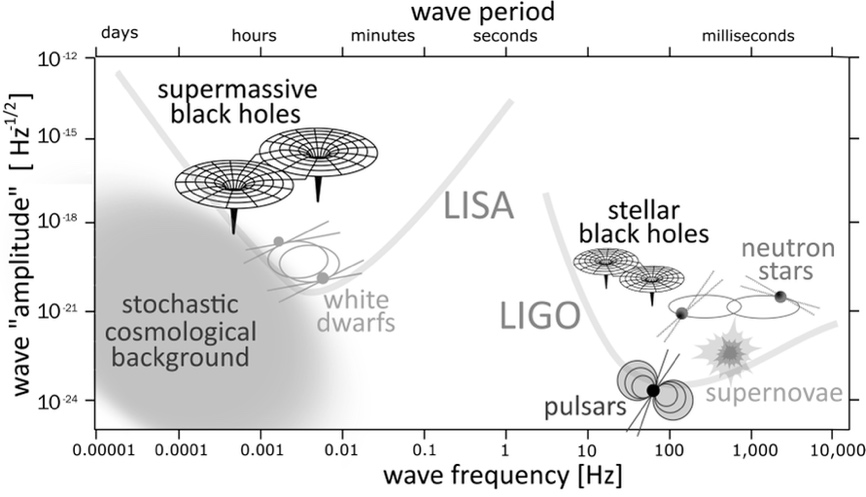
\includegraphics[width=0.88\linewidth,height=0.48\textheight,keepaspectratio]{../figs/source/en/fig-08-04.jpeg}

% DOCX paragraph 1223
\caption{\emph{Las diversas fuentes de ondas gravitatorias identificables por detectores como LIGO, Virgo o LISA\index{LISA}.}}\label{fig:08-04}
\end{figure}

% DOCX paragraph 1224
Obsérvese que las fuentes mostradas no están todas a la misma distancia de nosotros. Por el contrario, la amplitud característica indicada corresponde a fuentes en el límite del \emph{horizonte\index{observación!horizonte} de observación}, es decir, el volumen del universo dentro del cual se puede observar cada fuente. Este horizonte estará limitado a nuestra galaxia, a una distancia de unos cien kilopársecs, en el caso de la señal de ondas gravitatorias de una explosión de supernova. Sin embargo, será de decenas de megapársecs para sistemas binarios de estrellas de neutrones, e incluso de cientos de megapársecs para sistemas binarios de agujeros negros estelares. Por último, el horizonte de observación de LISA\index{LISA} incluirá gran parte del universo observable, ya que esencialmente «verá», aunque con distintas intensidades, todos los sistemas binarios de agujeros negros supermasivos que entren en su intervalo de frecuencias.

% DOCX paragraph 1225
La figura \ref{fig:08-04} reúne, por tanto, todas las fuentes de ondas gravitatorias que esperamos poder observar de manera realista. En realidad, en el fondo, todos los que trabajamos en este campo esperamos que en algún momento se mida una señal que no corresponda a ninguna de las que aparecen en la figura \ref{fig:08-04}. Detectar una fuente tan inesperada indicaría que hay algo incorrecto en nuestra descripción teórica de las fuentes de ondas gravitatorias. Pero, al mismo tiempo, ¡nos daría una excelente razón para ponerlo todo en cuestión!

% DOCX paragraph 1228
\section{La difícil vida de una pareja}\label{sec:08-couple}

% DOCX paragraph 1230
Tendemos a asociar la primera detección de ondas gravitatorias de un sistema binario con GW150914\index{GW150914}, el primer suceso que LIGO midió en 2015 y que correspondía a la fusión de un sistema binario de agujeros negros. Sin embargo, gracias a un trabajo iniciado 20 años antes, ya en la década de 1990 era evidente que Einstein tenía razón y que un sistema binario de objetos compactos produce ondas gravitatorias.

% DOCX paragraph 1231
Pero vayamos por orden. Hemos visto que el primer púlsar se descubrió en 1967 y que, desde entonces, se han observado estrellas de neutrones como púlsares aislados o en sistemas binarios, donde la estrella de neutrones\index{estrella de neutrones!binaria (véase)} emite rayos X\index{rayos X!radiación} al acretar materia de su compañera. Como más del 50 por ciento de las estrellas, y posiblemente hasta el 85 por ciento, no están aisladas, sino ligada\index{gravitatoriamente!ligada}s gravitatoriamente en sistemas binarios o triples, no se tardó mucho en concluir que un sistema binario podía contener dos estrellas de neutrones.

% DOCX paragraph 1232
Probablemente inspirados por consideraciones de este tipo, a principios de los años setenta los astrónomos estadounidenses Russell Hulse\index{Hulse, Russell} y Joseph Taylor\index{Taylor, Joseph} iniciaron una campaña sistemática de observaciones de púlsares que pudieran pertenecer a sistemas binarios. Utilizaron el radiotelescopio de Arecibo, en Puerto Rico, compuesto por 38\,000 paneles de aluminio alojados en una cavidad natural que formaban un reflector de ondas de radio de casi trescientos metros de diámetro. Pronto concentraron sus observaciones en el púlsar PSR B1913+16\index{PSR B1913+16}, descubierto en 1974.

% DOCX paragraph 1233
Sobre el papel, este púlsar no tiene nada de particular: una masa de 1,44 masas solares y un periodo de rotación de unos 60 milisegundos, lo que significa que gira sobre sí mismo 17 veces por segundo. Sin embargo, había algo anómalo en su emisión de radio, algo que no se había visto en ninguno de los púlsares conocidos hasta entonces. Para explicar ese comportamiento singular había que aceptar que la estrella orbitaba alrededor de una compañera; el problema era que esa compañera debería haber sido visible, y no lo era. Pero si la compañera también era una estrella de neutrones, las observaciones se explicaban bastante bien. Así fue como Hulse y Taylor descubrieron el primer sistema binario de estrellas de neutrones, conocido también como el \emph{púlsar binario de Hulse-Taylor}, pues es una binaria que contiene dos estrellas de neutrones, una de las cuales es un púlsar.

% DOCX paragraph 1234
Hoy, gracias a la enorme precisión de las observaciones radioastronómicas de púlsares, conocemos excepcionalmente bien PSR B1913+16\index{PSR B1913+16}. Por ejemplo, sabemos que las masas de las dos estrellas de neutrones son muy parecidas, 1,441 masas solares la primaria y 1,387 la secundaria, y que el periodo orbital es de 7,75 horas. Las órbita\index{Mercurio!órbita}s son elípticas, de modo que las dos estrellas giran alrededor del centro de masas común y su separación varía continuamente: alcanza unos 1,1 radios solares, 746\,600 km, en el punto de mínima separación, el periastro\index{periastro}\index{Mercurio!periastro}, y unos 4,8 radios solares, 3\,153\,600 km, en el de máxima separación, el apoastro\index{apoastro}. Dadas las masas y las elevadas velocidades orbitales de las estrellas, el púlsar binario PSR B1913+16 representa un sistema en el que los efecto\index{relativista!efecto}s relativistas se amplifican y, por tanto, son más fáciles de medir. Por ejemplo, al igual que la órbita de Mercurio, la del púlsar tampoco es cerrada, sino que experimenta un desplazamiento del periastro; recuérdese la figura 2.1. La diferencia crucial es que el periastro de PSR B1913+16 avanza 4,2 grados cada año, mientras que el de Mercurio avanza solo 0,4297 segundos de arco al año. En otras palabras, ¡la órbita de PSR B1913+16 varía en un solo día tanto como la de Mercurio en un siglo!

% DOCX paragraph 1235
El efecto\index{relativista!efecto} relativista más importante de PSR B1913+16\index{PSR B1913+16} está ligado a la emisión de ondas gravitatorias, que reduce la energía y el momento angular de la binaria y obliga a las dos estrellas a acercarse. En particular, su separación se reduce tres milímetros después de cada periodo, de modo que, al cabo de un año, ha disminuido unos 3,5 metros. En términos absolutos, la pérdida de energía de un sistema binario como PSR B1913+16 es enorme; además, el sistema está en nuestra galaxia y no demasiado lejos, a 21\,000 años luz. Y, sin embargo, la amplitud de las ondas gravitatorias producidas por la binaria es demasiado pequeña para detectores como LIGO y Virgo, diseñados para sistemas de frecuencias mucho más altas, como muestra la figura \ref{fig:08-04}. No obstante, la emisión de ondas gravitatorias es «visible» por los efectos que produce en la evolución de la órbita del púlsar y, en particular, por el cambio del instante en el que PSR B1913+16 debería alcanzar su periastro\index{periastro}.

% DOCX paragraph 1236
La figura \ref{fig:08-05} muestra el adelanto de la llegada de la binaria\index{estrella de neutrones!binaria (véase)} al periastro\index{periastro} en función del año en que se realizaron las observaciones. Es decir, la disminución del tiempo que necesita el púlsar para completar una órbita aparece representada mediante puntos y barras de error en la figura \ref{fig:08-05}. Obsérvese que los datos resumen observaciones realizadas durante 30 años y muestran claramente cómo el periodo orbital de PSR B1913+16\index{PSR B1913+16}, de aproximadamente siete horas y 45 minutos, ha disminuido casi 40 segundos en ese tiempo. Además, expresado en términos de la separación entre las dos estrellas de neutrones, ¡esta se ha reducido en 105 metros!

% DOCX paragraph 1237
\begin{figure}[htbp]
\centering
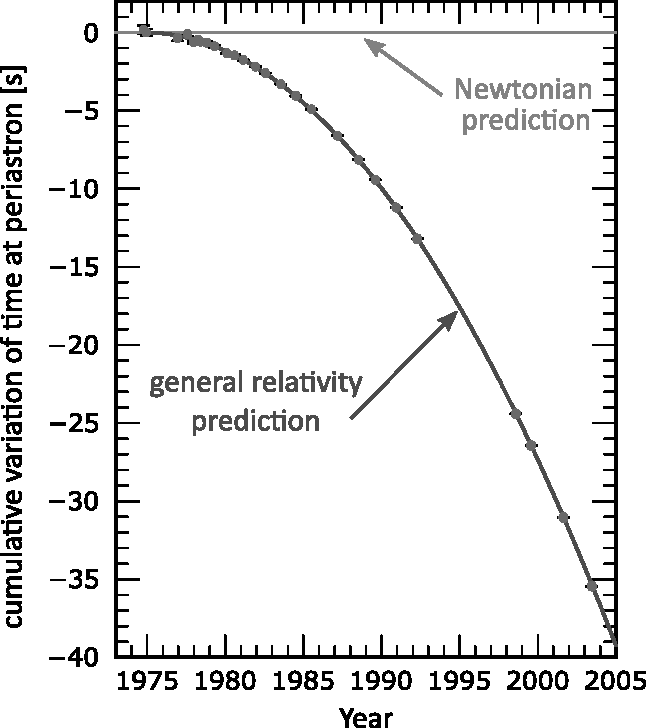
\includegraphics[width=0.88\linewidth,height=0.48\textheight,keepaspectratio]{../figs/pdf/en/fig-08-05.pdf}

% DOCX paragraph 1239
\caption{\emph{Observaciones del decaimiento de la órbita de PSR B1913+16\index{PSR B1913+16} en términos del adelanto del instante de paso por el periastro\index{periastro}. © datos de J. M. Weisberg y J. H. Taylor, ASP Conf. Series, 328, 25 (2005).}}\label{fig:08-05}
\end{figure}

% DOCX paragraph 1241
Este ejemplo pone de relieve una característica importante de los sistemas binarios y el título de esta sección. Independientemente de su naturaleza y su masa, una pareja de objetos astrofísicos ligados gravitatoriamente\index{gravitatoriamente!ligada} en un sistema binario está destinada, tarde o temprano, a\ldots{} ¡«colisionar»! En la inmensa mayoría de los casos, las escalas temporales de este proceso son enormes, mucho mayores que la edad del universo. Por ejemplo, para el sistema binario Tierra-Luna\index{Luna} se espera que la fusión tenga lugar dentro de 65 mil millones de años, por lo que no constituye un motivo de preocupación urgente. En cambio, las escalas temporales de los sistemas binarios de objetos compactos son mucho menores, del orden de unas decenas de millones de años. Ese plazo más corto nos permite «presenciar» estas colisiones.

% DOCX paragraph 1242
Las líneas continuas de la figura \ref{fig:08-05} corresponden, por su parte, a las predicciones teóricas según la teoría de la gravedad de Newton, una simple línea horizontal, pues no puede haber variación en una órbita cerrada, y según la relatividad general de Einstein. En este último caso, la curva no es horizontal porque la órbita debe cambiar, encogiéndose, debido a la emisión de ondas gravitatorias. Es notable la perfección con la que las medidas experimentales se ajustan a la curva teórica predicha por la relatividad general. Por esta razón, la observación de PSR B1913+16\index{PSR B1913+16} representa la primera prueba \emph{indirecta} de la existencia de ondas gravitatorias. Tras medir este proceso, Hulse y Taylor recibieron el premio Nobel de Física en 1993. Evidentemente, este resultado no resta mérito al trabajo de LIGO, cuya observación de GW150914\index{GW150914} proporcionó la primera prueba \emph{directa} de la existencia de ondas gravitatorias.

% DOCX paragraph 1243
Si lo que acabo de contar sobre las extraordinarias propiedades de PSR B1913+16\index{PSR B1913+16} deja atónito al lector y le lleva a imaginar dos estrellas de unos 25 kilómetros de diámetro que orbitan una alrededor de la otra a millones de kilómetros por hora, más vale que se prepare: ¡hay un sistema binario de púlsares aún más extremo! En 2003, utilizando el radiotelescopio del observatorio de Parkes\index{radiotelescopio!observatorio de Parkes}, en Australia, un equipo internacional coordinado por la astrónoma italiana Marta Burgay\index{Burgay, Marta} descubrió un sistema binario de dos púlsares, es decir, una binaria en la que ambas estrellas de neutrones son púlsares. El sistema se conoce como PSR J0737--3039\index{PSR J0737--3039}, y el mero hecho de que contenga dos púlsares permite extraer todavía más información. La separación en el apoastro\index{apoastro} de PSR J0737--3039 es comparable al radio solar, unos 800\,000 km, ¡y el periodo orbital es de tan solo 2,45 horas! Esta última propiedad es especialmente importante. Hemos visto que las órbitas de las dos estrellas difieren ligeramente de las predichas por la teoría de la gravedad de Newton. Estas diferencias se recogen en una serie de parámetros, conocidos como \emph{parámetros poskeplerianos\index{Kepler!parámetros poskeplerianos}\index{parámetros poskeplerianos}}, que sirven precisamente para medir cuánto difiere la órbita predicha por Einstein de la que predice Newton. Medirlos permite poner a prueba directamente la gravedad y comprobar la validez de las predicciones de Einstein. Como PSR J0737--3039 tiene un periodo orbital tan corto, nos brinda la oportunidad de recoger datos mucho más deprisa. De hecho, las mismas pruebas realizadas con PSR B1913+16 durante 30 años se llevaron a cabo con PSR J0737--3039 en menos de un tercio de ese tiempo. Por tanto, no es casualidad que, pocos años después de su descubrimiento, conozcamos muchos detalles de este fantástico sistema con una precisión increíble. En concreto, conocemos las masas de las dos estrellas, 1,3381 y 1,2489 masas solares; sus edades, 210 millones de años la más masiva y 50 millones la menos masiva; y sus periodos de rotación, uno corto de 22,7 milisegundos para la más vieja y otro «larguísimo» de 2,77 segundos para la más joven, que por esa razón también recibe el nombre de \emph{púlsar perezoso}\ldots{}

% DOCX paragraph 1244
Concluiré esta sección con una respuesta para quienes quizá tengan esta pregunta rondándoles la cabeza: si la separación entre las dos estrellas disminuye continuamente por la emisión de ondas gravitatorias, ¿cuándo se fusionarán las dos estrellas de neutrones de estos sistemas? Tal vez resulte decepcionante, pero aún no hace falta apuntarlo en la agenda. En efecto, la fusión de PSR B1913+16\index{PSR B1913+16} se espera dentro de unos 300 millones de años, y la de PSR J0737--3039\index{PSR J0737--3039} algo antes, dentro de unos 85 millones\ldots{} día arriba, día abajo\ldots{}

% DOCX paragraph 1247
\section[La aritmética de los agujeros negros binarios]{1 + 1 = 1: la extraña aritmética de los agujeros negros binarios}\label{sec:08-merger}

% DOCX paragraph 1249
Ya hemos establecido que los sistemas binarios de agujeros negros\index{sistemas binarios!agujeros negros}, los de estrellas de neutrones y los sistemas mixtos son las fuentes más intensas de ondas gravitatorias. Al menos a grandes rasgos, la génesis de estos sistemas está bastante clara.

% DOCX paragraph 1250
En primer lugar, como confirman abundantes datos de observación, las estrellas en sistemas binarios son más comunes que las aisladas. Además, sabemos que hay sistemas binarios compuestos por estrellas muy masivas que, mediante una explosión de supernova al final de su vida, pueden producir estrellas de neutrones o agujeros negros, dependiendo de la masa del núcleo en el momento del colapso. Por esta razón, no es difícil imaginar una trayectoria evolutiva del sistema binario en la que la estrella más masiva, la primaria, evoluciona más deprisa y es la primera que da lugar a una explosión de supernova, convirtiéndose en un agujero negro o una estrella de neutrones. Supongamos que las condiciones de la explosión son favorables. En ese caso, sobre todo si el retroceso generado por la explosión no es tan grande como para destruir el sistema binario, obtendremos una binaria compuesta por un objeto compacto, un agujero negro o una estrella de neutrones, y una estrella corriente de gran masa, la secundaria. Esta seguirá su trayectoria evolutiva, más lenta porque es menos masiva que la primaria, hasta que se produzca una segunda explosión de supernova cuyo remanente será, de nuevo, un agujero negro o una estrella de neutrones. Esta segunda explosión también pone en peligro la integridad del sistema binario, pero está claro que al menos una pequeña parte de estas binarias sobrevivirá «intacta» y dará lugar a sistemas binarios de objetos compactos, las fuentes ideales de ondas gravitatorias.

% DOCX paragraph 1251
Llegados a este punto, ¿qué ocurre? Para responder, nos centraremos primero en la evolución de un sistema binario compuesto por dos agujeros negros, que podemos dividir en tres fases: órbita casi circular; aproximación rápida en espiral; y caída final, fusión y oscilación amortiguada\index{agujero negro!oscilación amortiguada (ringdown)}, o \emph{ringdown}.

% DOCX paragraph 1252
En la primera fase, la de órbita casi circular, los dos objetos se mueven por trayectorias que serían exactamente circulares si no fuera por variaciones muy pequeñas ligadas a la pérdida de energía y momento angular mediante ondas gravitatoria\index{radiación!gravitatoria}s. Obsérvese que, incluso si las órbitas fueran inicialmente elípticas, como en el sistema binario PSR B1913+16\index{PSR B1913+16}, en este punto de la evolución se habrían vuelto casi circulares. Esto se debe a que la emisión intensa de ondas gravitatorias tiende a reducir su elipticidad y a «circularizar» las órbitas. La radiación\index{gravitatorio!radiación} gravitatoria emitida en esta fase puede durar millones o incluso decenas de millones de años, dependiendo de la separación inicial y de la masa de los componentes. Es esencialmente periódica y extremadamente débil, porque las velocidades no son altas. Además, estas ondas se emiten a frecuencias del orden de una millonésima de hercio, por lo que es imposible medirlas con los interferómetros actuales.

% DOCX paragraph 1253
En la segunda fase, la de aproximación rápida en espiral, los componentes de la binaria están destinados a acercarse inexorablemente en una danza cada vez más frenética. Sus órbitas se vuelven gradualmente menos circulares y adquieren cada vez más el aspecto de una espiral. Al mismo tiempo, al disminuir la separación entre los dos objetos, las ondas gravitatorias aumentan tanto en amplitud como en frecuencia. Como si estuviera inspirada en el \emph{Bolero} de Ravel, la aproximación avanza en un crescendo de ritmo e intensidad. Este aumento de la frecuencia y la amplitud de las ondas gravitatorias poco antes de la fusión se conoce también como «\emph{señal de gorjeo}», o \emph{chirp}, porque recuerda la manera en que las aves modulan su canto.

% DOCX paragraph 1254
En la última fase, que incluye algunas órbitas antes de que los agujeros negros se fusionen o «\emph{coalescan}», las ondas gravitatorias alcanzan su frecuencia y amplitud máximas, para amortiguarse rápidamente en cuanto se produce la fusión. En el caso de agujeros negros estelar\index{agujero negro!estelar}es, la frecuencia de la señal en esta fase final es del orden de cientos de hercios, es decir, de decenas de milésimas de segundo en términos del periodo. Sin embargo, es mucho menor, del orden de una centésima de hercio, con un periodo de aproximadamente un cuarto de hora, para agujeros negros supermasivos de alrededor de un millón de masas solares. Además, durante las últimas órbitas antes de la fusión, cuyo número exacto depende de la configuración del sistema binario, ocurre algo impresionante: la emisión de energía es tan copiosa que la cantidad perdida en esas últimas órbitas es comparable a la que se ha perdido desde la formación del sistema. En el caso de agujeros negros estelares, esta fase dura mucho menos que una fracción de segundo y, aun así, la energía perdida es comparable a la que la binaria ha emitido durante millones de años. La figura \ref{fig:08-06} ilustra un ejemplo de la compleja estructura geométrica de las ondas gravitatorias producidas en esta etapa final: muestra la señal emitida por un sistema de dos agujeros negros en fusión. En particular, los dos paneles muestran las dos polarizaciones de las ondas gravitatorias, «más» y «cruz», a izquierda y derecha, y el agujero negro final producido.\index{polarización}

% DOCX paragraph 1255
\begin{figure}[htbp]
\centering
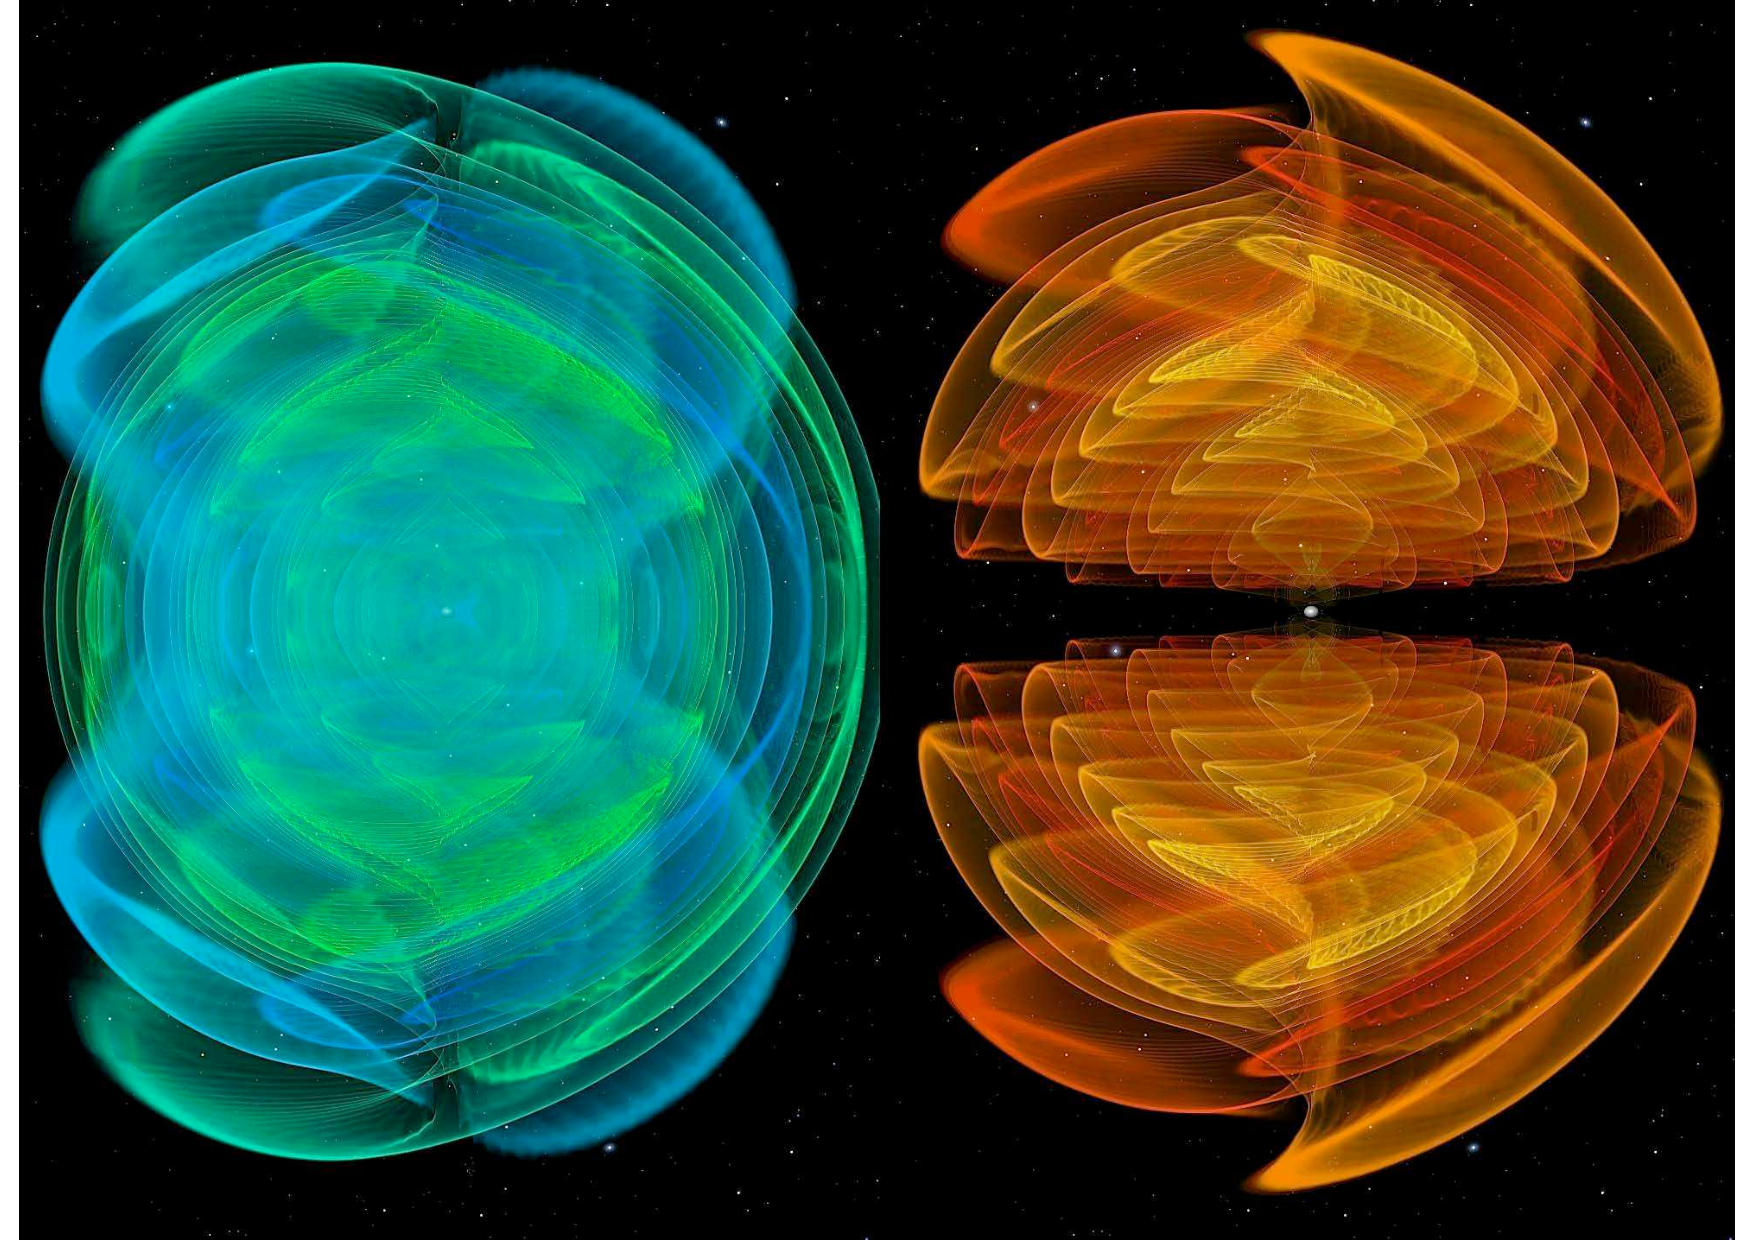
\includegraphics[width=0.88\linewidth,height=0.48\textheight,keepaspectratio]{../figs/pdf/en/fig-08-06.pdf}

% DOCX paragraph 1257
\caption{\emph{Ondas gravitatorias producidas por la fusión de un sistema binario de agujeros negros. © M. Koppitz / C. Reisswig / LR.}}\label{fig:08-06}
\end{figure}

% DOCX paragraph 1258
En el momento de la fusión, un único \emph{horizonte aparente} rodea y engloba los dos agujeros negros, todavía separados\textsuperscript{\hyperlink{note:08-05}{5}}. Este horizonte aparente común, que lo abarca todo, se forma cuando los dos agujeros negros están tan cerca que sus respectivos horizontes están a punto de tocarse. Debido a la aparición de ese horizonte común, un hipotético observador exterior nunca «vería» cómo los dos agujeros negros se tocan; evidentemente, me refiero a las regiones \emph{próximas} a los horizontes, ya que estos no son visibles por definición. Así se explica el enigmático título de esta sección, que resume en tono de humor todo el proceso de evolución: 1 (agujero negro) + 1 (agujero negro) = 1 (nuevo agujero negro).

% DOCX paragraph 1261
\section{Las fuentes de energía perfectas}\label{sec:08-energy}

% DOCX paragraph 1263
Curiosamente, el nuevo agujero negro producido por la fusión tendrá una masa comparable a la suma de las de los dos agujeros negros iniciales, pero algo menor. La diferencia se pierde en ondas gravitatorias, pues la energía\index{energia@energía!eficiencia de producción} que transportan equivale por completo a una masa, como nos recuerda la notable ecuación (3.2). Más interesante aún es que esa masa puede representar una buena fracción de la de los dos agujeros negros. Por ejemplo, en el caso de GW150914\index{GW150914}, los detectores LIGO midieron la forma de onda gravitatoria de un sistema binario de dos agujeros negros de 36 y 29 masas solares, que se fusionaron para producir un nuevo agujero negro de unas 62 masas solares. La parte que falta, ¡unas tres masas solares!, es la masa-energía radiada en forma de ondas gravitatorias en los últimos milisegundos. Si hacemos las cuentas, descubrimos que el sistema binario ha perdido el 5 por ciento de su masa en ondas gravitatorias o, si se prefiere, en distorsionar el rígido tejido del espaciotiempo que lo rodea. La proporción de masa perdida depende de las propiedades del sistema binario, la relación de masas y el espín de los agujeros negros, y puede alcanzar el 10 por ciento en el caso de agujeros negros con rotación máxima. Si pensamos ahora que la eficiencia energética de los procesos de fisión nuclear, como los que se utilizan en las centrales nucleares, es del orden del 0,1 por ciento, nos daremos cuenta enseguida de que la fusión de dos agujeros negros representa la manera más eficiente de producir energía en todo el universo. Esto también explica por qué estas fuentes son visibles a miles de millones de años luz.

% DOCX paragraph 1264
Esta enorme pérdida de energía nos ofrece una fascinante perspectiva de ciencia ficción. Quizá llegue un día en que nuestra civilización esté tan avanzada que pueda producir energía, no mediante la colisión de átomos pesados, como ocurre ahora en las centrales nucleares, sino mediante la colisión de agujeros negros microscópicos en alguna «central de energía\index{agujero negro!central de energía} de agujeros negros» situada a una distancia segura de nosotros, en el espacio interestelar. Entre otras cosas, una central así resolvería el problema de los residuos simplemente «dirigiendo» los productos de la colisión por una trayectoria que los alejara de nosotros. Algo que aún no he mencionado es que el agujero negro producido por la fusión suele adquirir una \emph{velocidad de retroceso\index{agujero negro!velocidad de retroceso (kick)}}, también llamada \emph{kick}, o «patada». Por tanto, si el agujero negro producido tiene carga y retrocede, se puede desviar fácilmente y dirigir adonde queramos mediante campos magnéticos. Es una digresión claramente de ciencia ficción, pero con una base científica correcta. En cualquier caso, ¡mejor no intentarlo en casa!

% DOCX paragraph 1265
Volvamos a los agujeros negros reales, astrofísicos. En relatividad general, y salvo en situaciones muy particulares, el agujero negro final producido por la fusión de un sistema binario de agujeros negros es del tipo Kerr\index{agujero negro!Kerr}, por tanto, está en rotación. La velocidad de rotación y la dirección del vector de espín dependen de las propiedades iniciales de los dos agujeros negros, en particular de su relación de masas y sus espines. Sin embargo, al nacer, el objeto compacto no es un agujero negro de Kerr\index{agujero negro!Kerr} plenamente formado, sino uno «perturbado». Lo que ocurre entonces es muy interesante: el agujero negro perturbado es capaz de «sacudirse» todas las imperfecciones ligadas a su violenta formación, de modo que en unos pocos milisegundos, al menos en el caso de un agujero negro estelar, todas las perturbaciones se irradian, es decir, se pierden mediante la emisión de ondas gravitatorias. Así, el agujero negro recién formado se asienta rápidamente en su configuración final, también llamada asintótica. La señal de ondas gravitatorias emitida durante estas «sacudidas» tiene un nombre muy particular: la \emph{oscilación amortiguada\index{agujero negro!oscilación amortiguada (ringdown)}}, o \emph{ringdown}, del agujero negro. Como decae exponencialmente, es una señal muy breve y evanescente, parecida al sonido que emite una campana cuando el badajo la «perturba» suavemente.

% DOCX paragraph 1266
Conviene subrayar que, al igual que cada campana tiene un sonido específico relacionado con sus propiedades, su masa, forma, aleación metálica, etc., un agujero negro tiene una señal de oscilación amortiguada estrechamente ligada a sus propiedades: la masa y el espín. Por eso, poder medir esta señal en la fusión de un sistema binario de agujeros negros es esencial: recoge de forma única información sobre las propiedades del agujero negro que no sería accesible de otro modo. Además, permite confirmar que el producto de la fusión es realmente un agujero negro y no otra cosa. Por desgracia, medir esta señal, cuya amplitud es intrínsecamente evanescente, no es nada fácil. Aun así, ya se ha hecho, por ejemplo con LIGO y Virgo en GW150914\index{GW150914}, y la medida sirvió para descartar que el objeto producido por aquella fusión fuera una gravastar\index{gravastar}.

% DOCX paragraph 1269
\section{Un desafío teórico formidable}\label{sec:08-numerics}

% DOCX paragraph 1271
Tal vez, llegados a este punto, los lectores se pregunten: «Pero ¿cómo sabemos todas estas cosas?». Pues bien, porque las calculamos numéricamente casi diez años antes de que se detectara la primera señal de ondas gravitatorias. Desde la década de 1990, un gran grupo de físicos teóricos de todo el mundo ha desarrollado algoritmos avanzados y construido sofisticados códigos numéricos capaces de aprovechar los potentes recursos de los superordenadores\index{superordenadores} paralelos. Este esfuerzo ha dado lugar al nacimiento de una nueva rama de la física, la \emph{relatividad numérica\index{relatividad numérica}}, cuyo propósito es resolver las ecuaciones de Einstein numéricamente, a menudo junto con las de la hidrodinámica\index{relativista!hidrodinámica} relativista o la magnetohidrodinámica, para describir con la máxima precisión posible la evolución de un sistema binario de agujeros negros o estrellas de neutrones. Sin embargo, el objetivo no tiene nada de trivial, pues las ecuaciones de la relatividad general, que describen la dinámica de estos objetos, figuran entre las más complejas que se conocen, y la presencia de fuertes no linealidades y singularidades convierte la búsqueda de la solución en un verdadero desafío. De hecho, durante muchos años se avanzó lentamente en esta área de investigación, entre repetidos fracasos y frustraciones, hasta el punto de que a finales de los años noventa nadie creía que la relatividad numérica llegara a calcular algo útil.

% DOCX paragraph 1272
Esta opinión dio lugar a una famosa apuesta entre Kip Thorne\index{Thorne, Kip}, galardonado con el premio Nobel de Física en 2017, y una docena de científicos dedicados a investigar en relatividad numérica, entre ellos yo. La apuesta consistía en quién lograría antes un avance: Kip apostaba a que LIGO mediría la señal de fusión de un sistema binario de agujeros negros antes de que nosotros, los teóricos, pudiéramos calcularla mediante simulaciones de relatividad numérica. Estaba en juego una botella de vino. Sin duda, Kip pretendía animarnos, ¡y funcionó! Las primeras señales teóricas de ondas gravitatorias producidas por un sistema binario de agujeros negros se calcularon numéricamente en 2005. Y la primera señal experimental se midió diez años después, en 2015, con GW150914\index{GW150914}. Kip Thorne\index{Thorne, Kip} aceptó deportivamente la derrota e incluso la mencionó en su conferencia Nobel, celebrada en Estocolmo el 8 de diciembre de 2017.

% DOCX paragraph 1273
Durante los últimos 15 años se han logrado avances notables mediante cálculos analíticos para las primeras fases de la dinámica de la binaria y simulaciones numéricas para las etapas finales, más no lineales y difíciles de calcular. Gracias a estos avances, los sistemas binarios de objetos compactos son hoy las fuentes de ondas gravitatorias que mejor comprendemos.

% DOCX paragraph 1274
Permítanme insistir: poder calcular la señal de ondas gravitatorias tiene una relevancia que va mucho más allá de resolver un problema matemático difícil. El conocimiento teórico de la señal es esencial para detectar estas fuentes, porque, aunque liberan enormes cantidades de energía en forma de ondas gravitatorias, suelen encontrarse a distancias considerables de la Tierra. Por ello, la amplitud de sus ondas gravitatorias es mínima, como ya hemos mencionado varias veces.

% DOCX paragraph 1275
Estas mediciones están claramente en el límite de nuestra tecnología. De ahí que detectar ondas gravitatorias represente un auténtico «desafío», tanto para la física experimental como para la teórica. Si se tiene todo en cuenta, incluida la intensidad de la señal emitida, la distancia de la fuente, el ruido del detector, etc., la señal que realmente se mide suele ser comparable al ruido de fondo de los detectores. Por tanto, es prácticamente imposible medirla; en la jerga técnica se dice que, en estas condiciones, la relación señal-ruido\index{relación señal-ruido}\index{ruido!relación señal-ruido} es del orden de la unidad. Ahora bien, si conociéramos la señal de antemano, en principio sería posible «extraerla» del ruido de fondo mediante una técnica llamada \emph{filtrado adaptado\index{ruido!filtrado adaptado}}. Para hacerse una idea de lo que significa, imagine el lector que escucha una emisión de radio con mucho ruido en la que, pese al crepitar, aún se distinguen algunas palabras. Si dispusiéramos de cierta información básica, como el idioma, el tema del que se habla, el número de voces ante el micrófono, etc., nuestro cerebro sería capaz de «extraer» la señal del ruido y reconstruir casi por completo lo transmitido. Lo que sucede con las ondas gravitatorias y los filtros adaptados\index{filtros adaptados} no es muy distinto: el conocimiento previo permite a los detectores revelar incluso una señal muy tenue. Así comenzó, hace más de 20 años, el formidable desafío teórico de calcular con la máxima precisión posible las formas de onda gravitatoria producidas por las fuentes más comunes, en todas sus configuraciones posibles, y proporcionar esa información a los científicos que trabajan en la detección de señales y el análisis de datos. A día de hoy, el desafío aún no ha terminado. El conocimiento teórico previo de la señal permite comparar la señal experimental mezclada con el ruido del detector, eliminar este último por filtrado y encontrar así la señal de ondas gravitatorias incluso cuando la relación señal-ruido\index{relación señal-ruido}\index{ruido!relación señal-ruido} es muy baja.

% DOCX paragraph 1276
Puede parecer una tarea sencilla, ¡pero no lo es! A pesar de los enormes avances desde 2005, resolver las ecuaciones\index{ecuaciones!diferenciales} de Einstein sin aproximaciones ni simetrías sigue siendo un grandísimo reto. A su enorme complejidad hay que sumar la de las ecuaciones de la hidrodinámica y la magnetohidrodinámica, necesarias para describir el movimiento de la materia y cuya resolución en condiciones realistas plantea un desafío comparable. El conjunto de ecuaciones diferenciales en derivadas parciales acopladas que hay que resolver es tan grande que solo se puede obtener una solución numérica aprovechando los recursos de los superordenadores\index{superordenadores} paralelos más potentes. A pesar de todas estas dificultades y problemas, a cuya solución he dedicado buena parte de mi carrera, la predicción de las ondas gravitatorias procedentes de fuentes compactas nunca ha sido tan exacta y precisa. Todos estos esfuerzos han sellado una formidable colaboración entre teoría y experimentación con el objetivo común de detectar ondas gravitatorias, y han mostrado hasta dónde podemos llegar al combinar nuestras fuerzas.

% DOCX paragraph 1279
\section{Para terminar, puro asombro}\label{sec:08-luminosity}

% DOCX paragraph 1281
A estas alturas, el lector ya se habrá dado cuenta de que no puedo evitar usar ecuaciones de vez en cuando\ldots{} Cerraré, pues, esta sección volviendo por un momento a la ecuación \eqref{eq:08-01} y, en particular, a la expresión de la derecha. Soy plenamente consciente de que lo que hago ahora contradice directamente lo que he venido afirmando: necesito que la atención de los lectores se centre en las constantes que aparecen en el lado derecho de la ecuación \eqref{eq:08-01}. Sí, esas mismas constantes que siempre he recomendado ignorar porque no son importantes. Haré incluso algo más: para dejar más claro este cambio de enfoque, solo por esta vez, señalaré en negro las constantes físicas \emph{c} y \emph{G}, y dejaré todo lo demás en gris. Así, la parte de la ecuación \eqref{eq:08-01} que ahora nos interesa queda como sigue:

% DOCX paragraph 1283
\begingroup\renewcommand{\theHequation}{8.repeat}\begin{equation}\tag{8.1}\label{eq:08-01-repeat}
L_{GW} \simeq \frac{c^{5}}{G}\textcolor{gray}{\left( \frac{r_{s}}{R} \right)^{2}\left( \frac{v}{v} \right)^{6}\ }
\end{equation}\endgroup

% DOCX paragraph 1285
Consideremos una fuente de ondas gravitatorias cuyas dimensiones sean iguales al radio de Schwarzschild correspondiente y que se mueva a una velocidad próxima a la de la luz, como ocurre cuando dos agujeros negros están a punto de fusionarse. En este caso tendremos \emph{r\textsubscript{s}/R} ≃ 1 y \emph{v/c} ≃ 1, de modo que las partes grises de la ecuación \eqref{eq:08-02} son aproximadamente iguales a uno, y la ecuación depende en la práctica solo de las constantes, quedando reducida a

% DOCX paragraph 1287
\begin{equation}\label{eq:08-02}
L_{GW}\sim\frac{c^{5}}{G}\sim 3{,}6 \times 10^{48}\ \mathrm{vatios}
\end{equation}

% DOCX paragraph 1289
La luminosidad en ondas gravitatorias\index{luminosidad!ondas gravitatorias} es sencillamente inmensa, gigantesca, colosal. Basta pensar que en el universo hay aproximadamente cien mil millones (10\textsuperscript{11}) de galaxias, cada una con cien mil millones de estrellas, otro factor 10\textsuperscript{11}, y que cada estrella tiene una luminosidad de 10\textsuperscript{26} vatios. Con la ecuación \eqref{eq:08-02} acabamos de descubrir que, en el momento de la fusión, un sistema binario de agujeros negros irradia tanta energía como la que se emite durante el mismo tiempo en forma de ondas electromagnéticas en todo el universo. No sé cómo se sentirá quien esté leyendo estas líneas; yo, cada vez que lo pienso, me quedo sumido en el más puro asombro.

% DOCX paragraph 1292
\section[Dinámica de las estrellas de neutrones binarias]{La compleja dinámica de las estrellas de neutrones binarias}\label{sec:08-neutron-stars}

% DOCX paragraph 1294
La dinámica de un sistema binario de estrellas de neutrones\index{sistema binario!estrellas de neutrones} guarda muchas similitudes con la de los agujeros negros binarios, pero también algunas diferencias fundamentales. Procedamos, pues, con orden y volvamos a clasificar las fases de la dinámica, que por lo general son cuatro: órbita casi circular; aproximación rápida en espiral; fusión y posfusión\index{posfusión}; y colapso y acreción.\index{estrella de neutrones!binaria (véase)}

% DOCX paragraph 1295
La fase de órbita casi circular es prácticamente idéntica a la que ya hemos comentado para los agujeros negros. Ambos sistemas se pueden describir con las mismas ecuaciones, tratando los componentes de la binaria como partículas puntuales.

% DOCX paragraph 1296
La dinámica de la segunda fase, la aproximación rápida en espiral, también es muy parecida a la de un sistema de agujeros negros, pero no idéntica. Explicaré por qué. En primer lugar, las estrellas de neutrones son más grandes que un agujero negro de la misma masa. Por ejemplo, hemos visto que una estrella de neutrones típica tiene una masa de 1,4 masas solares y un radio de unos 12 kilómetros, mientras que un agujero negro de la misma masa tiene un radio de Schwarzschild de unos 4,2 kilómetros. Así pues, manteniendo la masa, un sistema binario de estrellas de neutrones se fusionará antes que uno de agujeros negros, simplemente porque las estrellas llegarán a «tocarse» cuando la separación entre los dos objetos sea del orden de 24 kilómetros, en lugar de ocho. En segundo lugar, como las estrellas de neutrones están hechas de materia, pueden deformarse por las mareas y, por tanto, seguir trayectorias ligeramente distintas de las de agujeros negros de la misma masa. Este último punto es especialmente importante, por lo que intentaré explicarlo con más detalle. Hemos visto que un campo gravitatorio no uniforme, es decir, un campo gravitatorio normal, genera fuerzas de marea\index{fuerzas de marea} que alteran los objetos deformables, como el agua de la superficie terrestre, que puede elevarse bajo el campo de marea de la Luna\index{Luna}. Un sistema binario de objetos compactos genera un campo gravitatorio no uniforme, ya que la curvatura entre los dos objetos es mayor que en las regiones más lejanas. Por tanto, un objeto deformable situado en ese campo gravitatorio cambiará de forma. Como un agujero negro representa el límite de intensidad del campo gravitatorio, no es deformable. Lo expresamos diciendo que su coeficiente de deformabilidad de marea, también llamado \emph{número\index{Love!número} de Love}, es cero\textsuperscript{\hyperlink{note:08-06}{6}}. Dicho de otro modo, podemos suponer que un agujero negro esférico seguirá siendo esférico aunque se sitúe muy cerca de otro agujero negro en un sistema binario. He aquí la diferencia crucial: con una estrella de neutrones no sucede lo mismo. Una estrella de neutrones que es esférica cuando está aislada adquirirá una forma deformada, no esférica, en presencia de otra estrella de neutrones.

% DOCX paragraph 1297
Este cambio de forma es muy significativo por dos razones. La primera es que induce cambios en las órbitas de las estrellas de neutrones respecto a las de agujeros negros de la misma masa. Por tanto, en igualdad de condiciones, las ondas gravitatorias producidas por estrellas de neutrones durante la aproximación rápida en espiral serán distintas de las correspondientes ondas producidas por agujeros negros. De hecho, es precisamente ese comportamiento diferente el que nos permite distinguir, una vez conocida la masa, si el objeto compacto es un agujero negro o una estrella de neutrones\textsuperscript{\hyperlink{note:08-07}{7}}. La segunda razón es aún más importante: la deformabilidad de marea de las estrellas de neutrones, es decir, cuánto pueden deformarse en un campo gravitatorio no uniforme, depende de su composición interna. Por tanto, en principio se puede determinar su ecuación de estado\index{ecuación de estado} simplemente analizando las ondas gravitatorias en las últimas etapas de la aproximación en espiral, cuando las dos estrellas están más cerca y los efectos de marea son más intensos. Esto es exactamente lo que hicieron LIGO y Virgo con GW170817\index{GW170817}, que proporcionó las primeras restricciones experimentales, aunque todavía bastante inciertas, sobre la deformabilidad de marea de las estrellas de neutrones.

% DOCX paragraph 1303
\section{Una batalla fatal contra la gravedad}\label{sec:08-remnant}

% DOCX paragraph 1305
La dinámica de la tercera fase, la fusión y la posfusión\index{posfusión}, es decididamente distinta de lo que hemos visto para los agujeros negros. Cuando dos estrellas de neutrones se fusionan, por lo general no producen un agujero negro, sino un tipo particular de estrella: una estrella de neutrones \emph{hipermasiva}, o HMNS\index{HMNS (estrella de neutrones hipermasiva)}. El adjetivo «hipermasiva» deriva de que la masa de este objeto, la suma de las masas de las dos estrellas iniciales menos la que se pierde en la colisión, de la que hablaremos más adelante, supera la masa máxima que hemos visto que existe para las estrellas de neutrones; recuérdese la figura 5.6 del capítulo 5. Esta estrella hipermasiva está en equilibrio, pero es un equilibrio muy precario, que puede perder con facilidad. Por eso decimos que se encuentra en un \emph{equilibrio metaestable\index{equilibrio!metaestable}}. En esencia, el campo gravitatorio es tan intenso, pues la estrella hipermasiva tiene casi el doble de masa que las originales, que está a punto de colapsar en un agujero negro. Sin embargo, consigue evitar el colapso, al menos provisionalmente, rotando muy deprisa y de manera diferencial: más despacio en el núcleo y más deprisa en las capas externas. En otras palabras, la estrella hipermasiva producida por la colisión libra una batalla desesperada contra la gravedad, estableciendo un precario equilibrio en el que distribuye su materia y rota casi a la máxima velocidad posible.\index{diferenciales!rotación}

% DOCX paragraph 1306
Por desgracia para la estrella, no puede mantener ese precario equilibrio mucho tiempo, porque rota tan deprisa que ni siquiera es axisimétrica. En cambio, está deformada y se parece a un enorme «cacahuete en rotación». En esta configuración pierde energía y momento angular mediante la emisión de ondas gravitatorias. Esa pérdida conducirá inevitablemente al colapso\index{gravitatorio!colapso} gravitatorio en un agujero negro en rotación. No es fácil estimar cuánto puede prolongar la estrella hipermasiva su batalla contra la gravedad. Este delicadísimo equilibrio depende de forma no lineal de una serie de factores, como la masa de la binaria, la diferencia de masas entre las dos estrellas de neutrones, la ecuación de estado y la intensidad del campo magnético. Solo las simulaciones numéricas permiten describir con precisión esta fase, demasiado dinámica y no lineal para aproximarla mediante tratamientos analíticos o perturbativos. De estas simulaciones hemos aprendido que, según las condiciones físicas mencionadas, la estrella hipermasiva puede sobrevivir solo decenas de milisegundos, en el caso de masas iniciales muy altas, o varios cientos de milisegundos. En general, sin embargo, parece muy difícil que sobreviva más de unos pocos segundos, al menos para estrellas de neutrones típicas con masas iniciales de 1,3--1,4 masas solares.

% DOCX paragraph 1307
Durante su breve vida, la estrella hipermasiva realiza dos tareas esenciales. La primera es lanzar grandes cantidades de materia al espacio interestelar en forma de vientos de alta energía, un fenómeno del que hablaremos después con más detalle. La segunda, quizá aún más importante, es emitir grandes cantidades de ondas gravitatorias\index{espectro!ondas gravitatorias}, precisamente porque se parece mucho a un cacahuete que rota deprisa y, por tanto, se aleja mucho de la forma esférica. Esta emisión de ondas gravitatorias se produce a frecuencias precisas y casi constantes, relacionadas con las propiedades de la estrella hipermasiva, básicamente su masa y su ecuación de estado\index{ecuación de estado}. La emisión queda impresa en el llamado \emph{espectro de ondas gravitatorias\index{posfusión!espectro de ondas gravitatorias} de posfusión}, la distribución de la energía perdida en ondas gravitatorias en función de su frecuencia. Las características de ese espectro son como una huella dactilar: en principio, bastaría observar las principales frecuencias que lo caracterizan para obtener información sobre el «santo grial» de la física nuclear, la ecuación de estado de la materia a densidades nucleares.

% DOCX paragraph 1308
Por desgracia, las perspectivas de observar ese espectro de posfusión\index{posfusión!espectro de ondas gravitatorias}\index{posfusión} no son muy buenas, al menos con los detectores interferométricos actuales. La frecuencia de la señal de ondas gravitatorias, ya muy alta poco antes de la fusión, alrededor de 1 kHz, aumenta aún más durante la posfusión, hasta unos 2--3 kHz. En la práctica, la señal medida a estas frecuencias y para fuentes a las distancias típicas esperadas para estrellas de neutrones binarias es demasiado débil y está dominada por el ruido. Como resultado, interferómetros como LIGO y Virgo son prácticamente «sordos» a esas frecuencias. Es lo que ocurrió con GW170817\index{GW170817}, que permaneció visible para los detectores LIGO durante un tiempo antes de la fusión, pero cuya señal desapareció pronto porque sus frecuencias eran demasiado altas para medirlas. Afortunadamente, estas sombrías perspectivas cambiarán radicalmente con la construcción de detectores interferométricos de «tercera generación», como el Telescopio Einstein y Cosmic Explorer\index{Cosmic Explorer}, diseñados para ser mucho más sensibles en la región de 2--3 kHz. Cuando estos detectores entren en funcionamiento, dentro de unos 15 años, por fin será posible medir esta señal de alta frecuencia, débil pero de enorme importancia.

% DOCX paragraph 1309
¿Qué ocurre cuando se pierde la batalla? Una vez que la estrella hipermasiva ha perdido demasiada energía de rotación\index{energia@energía!de rotación} y ha agotado su capacidad de resistir a la gravedad, se ve obligada a colapsar en un agujero negro. Sin embargo, el horizonte de sucesos del agujero negro resultante no absorbe toda su materia. Esto es posible porque la estrella hipermasiva es relativamente grande y solo su núcleo interno colapsa en un agujero negro. Cuando eso sucede, las partes externas están a una distancia considerable del centro, de hasta 15--20 kilómetros. Como el horizonte de sucesos producido tiene un radio de unos ocho kilómetros, parte de la materia de la estrella acaba en órbitas estables y, por tanto, el agujero negro no la captura. Bueno, al menos no de inmediato. En ese momento, el sistema resultante del colapso\index{gravitatorio!colapso} de la estrella hipermasiva está compuesto por un agujero negro rodeado de materia de alta densidad y temperatura que orbita a su alrededor. En esencia, constituye un disco de acreción geométricamente grueso, también llamado «toro\index{disco de acreción!toro} de acreción». Para hacerse una idea mejor de lo que ocurre tras la fusión, recomiendo visitar mi página web y buscar la sección dedicada a visualizar las simulaciones numéricas de mi grupo de investigación. Creo que una visualización vale más que mil palabras para explicar la compleja fusión de un sistema binario de estrellas de neutrones\ldots{}

% DOCX paragraph 1310
Como los lectores pueden imaginar, el toro de acreción tampoco está destinado a durar mucho. Su materia está muy magnetizada y sujeta a inestabilidades, en particular la inestabilidad magnetorrotacional\index{inestabilidad!magnetorrotacional}, que desencadenan su acreción sobre el agujero negro. Así, pocos segundos después de su creación, toda la materia del toro es absorbida por el agujero negro, que queda como único verdadero testigo de todo el proceso de fusión del sistema binario de estrellas de neutrones. Una vez más, la extraña aritmética de estos sistemas puede resumirse así: 1 (estrella de neutrones) + 1 (estrella de neutrones) = 1 (agujero negro)\textsuperscript{\hyperlink{note:08-08}{8}}.

% DOCX paragraph 1313
\section{Un misterio que comenzó con la Guerra Fría}\label{sec:08-gamma}

% DOCX paragraph 1315
Una diferencia muy importante entre la fusión de agujeros negros binarios y la de estrellas de neutrones binarias es que de estas últimas se espera, por lo general, una contrapartida electromagnética\index{contrapartida electromagnética}\index{radiación!electromagnética}. Es una expectativa natural si pensamos que la fusión de estrellas de neutrones consiste esencialmente en una colisión, a velocidades próximas a la de la luz, de dos concentraciones masivas y compactas de materia. Es casi inevitable que un proceso de este tipo, con las altas densidades y temperaturas que produce, genere una señal relacionada con la radiación electromagnética. No obstante, para entender esta señal tengo que contar un misterio que comenzó en los años setenta, en plena Guerra Fría.

% DOCX paragraph 1316
En aquellos años, los dos bloques competían encarnizadamente tanto en armamento como en desarrollo tecnológico. Por razones que hoy parecen más que obvias, pero entonces no lo eran, ambos habían acordado prohibir todos los ensayos de bombas nucleares. En ese contexto de no proliferación de armas nucleares, mezclado con la desconfianza general entre las dos superpotencias, en los años setenta Estados Unidos lanzó un satélite espía capaz de recoger radiación en la banda de los rayos gamma. Era un satélite muy distinto de como podríamos imaginarlo: en lugar de apuntar al cielo, apuntaba permanentemente a la Tierra y, en particular, exploraba el vasto territorio de la Unión Soviética. Su propósito era bastante obvio: detectar las señales de rayos gamma producidas por una explosión nuclear. Dicho de otro modo, se había construido para medir destellos de rayos gamma. Lo paradójico de esta historia de espías es que el satélite no registró ningún suceso terrestre, porque los soviéticos respetaron la prohibición de los ensayos nucleares. Al mismo tiempo, no fue un desperdicio total de tecnología. Al contrario: registró una serie de destellos de rayos gamma muy intensos y de procedencia claramente celeste. Como estos resultados estaban protegidos por el secreto militar, la comunidad científica sabía muy poco de ellos. De hecho, hicieron falta muchos años para desclasificar las observaciones, y muchos más para que resultara evidente la importancia de estas misteriosas fuentes de destellos de rayos gamma. Hubo que esperar hasta principios de los años noventa para que se desarrollara plenamente la investigación astronómica en este campo.

% DOCX paragraph 1317
Hoy, tras unos treinta años de observaciones del «cielo de rayos gamma\index{astronomía!rayos gamma}», o astronomía de rayos gamma, sabemos que, junto a las fuentes galácticas y extragalácticas cuyas propiedades conocemos mediante mediciones repetidas, hay otras dos clases de fuentes tan interesantes como misteriosas. En primer lugar, son fuentes \emph{episódicas}, en el sentido de que solo se observan una vez y durante periodos muy breves. Por eso se llaman \emph{brotes de rayos gamma\index{brotes de rayos gamma}}, o GRB\index{GRB|see{brotes de rayos gamma}}, por sus siglas en inglés. Como estos destellos son muy breves, episódicos, aparecen sin precursores en otras bandas y no se pueden medir más de una vez, sigue habiendo mucha incertidumbre sobre las fuentes que los generan. Sí sabemos que se dividen en dos grandes clases: brotes \emph{largos\index{brotes de rayos gamma!largos}} y \emph{cortos\index{brotes de rayos gamma!cortos}}. Pese al nombre, incluso los largos son extremadamente breves: duran entre un par de segundos y aproximadamente un minuto. Los cortos, por su parte, duran mucho menos, entre una fracción de segundo y unos dos segundos. Por supuesto, no siempre es fácil distinguir los brotes cortos, que representan alrededor del 30 por ciento del total, de los largos. Sin embargo, al estudiar las estadísticas de todos los brotes de rayos gamma observados hasta ahora, unos 2300, con una media actual de uno observado cada día, queda claro que hay dos poblaciones distintas: una con una duración media de unos 0,3 segundos, la de los brotes \emph{cortos}, y otra de unos 30 segundos, la de los \emph{largos}.

% DOCX paragraph 1318
En ambos casos se trata de fenómenos explosivos que liberan enormes cantidades de energía\index{energia@energía!eficiencia de producción}, del orden de 10\textsuperscript{50}--10\textsuperscript{52} erg, en unos pocos segundos o menos. Además, las observaciones indican claramente la presencia de un chorro colimado que se propaga a velocidades relativistas y produce radiación de rayos gamma durante su propagación o cuando colisiona con el medio interestelar. Para hacerse una idea de la enormidad de la energía que liberan estos objetos, pensemos en lo siguiente: ¡en unos segundos, los brotes de rayos gamma liberan tanta energía como todas las estrellas de nuestra galaxia, que suman billones, en un año entero! Precisamente por eso son visibles a distancias inmensas, incluso desde los rincones más remotos del universo. Considerando las energías en juego, que se produzcan tan lejos es algo positivo: recibir uno solo de estos destellos podría suponer el fin de buena parte de la vida en nuestro planeta\ldots{}

% DOCX paragraph 1319
No sorprenderá saber que no escasean, de hecho sobran, los modelos teóricos capaces de explicar de manera más o menos satisfactoria la fenomenología observada en los brotes de rayos gamma. Dejando de lado las hipótesis más imaginativas y exóticas, la comunidad científica actual coincide en asociar los brotes largos con la implosión de estrellas especialmente masivas. En este escenario, el colapso del núcleo estelar genera un agujero negro que acreta materia del interior de la estrella mediante un disco de acreción y lanza un chorro\index{relativista!chorro} lo bastante potente como para atravesar el resto de la estrella y emerger, haciéndose visible.\textsuperscript{\hyperlink{note:08-09}{9}}

% DOCX paragraph 1320
A finales de los años ochenta se propuso una explicación plausible de los brotes cortos\index{brotes de rayos gamma!cortos} de rayos gamma basada en la fusión de un sistema binario de estrellas de neutrones.\textsuperscript{\hyperlink{note:08-10}{10}} La hipótesis parecía perfectamente razonable desde el principio. Las escalas temporales asociadas a la fusión de una binaria de estrellas de neutrones son precisamente del orden de 0,1--1 segundos, y el sistema binario dispone de enormes reservas de energía gravitatoria. Bastaría liberar unos pocos puntos porcentuales de esa energía para explicar las luminosidades medidas en los brotes cortos de rayos gamma. Pese a lo plausible del modelo y a los cientos de brotes cortos observados durante los últimos treinta años, la confirmación de esta hipótesis no llegó hasta 2017, gracias a un suceso del que ya hemos hablado: GW170817\index{GW170817}.

% DOCX paragraph 1323
\section{Mucho más que fuentes de ondas gravitatorias}\label{sec:08-multimessenger}

% DOCX paragraph 1325
Ya he mencionado que la señal de ondas gravitatorias de GW170817\index{GW170817} se interrumpió bruscamente en el momento de la fusión de las dos estrellas. Sin embargo, no he contado que poco después ocurrió algo asombroso. Tan solo 1,74 segundos después de desaparecer del canal de ondas gravitatorias, ¡GW170817 «reapareció» en el canal electromagnético como un brote corto de rayos gamma: GRB 170817A\index{GRB 170817A}! Se pudieron combinar los tiempos de llegada de la señal de ondas gravitatorias a los dos detectores LIGO y tener en cuenta que Virgo\index{Virgo} no la había visto, aunque en teoría podría haberlo hecho. Los científicos de la colaboración LIGO/Virgo localizaron enseguida la región del cielo, grande pero no inmensa, de la que procedía la señal y que correspondía al \emph{punto ciego\index{detector de ondas gravitatorias!punto ciego}} de Virgo, es decir, la región a la que no era sensible en ese momento.\textsuperscript{\hyperlink{note:08-11}{11}} Así, pocos segundos después de detectar GW170817, decenas de telescopios y satélites apuntaron en la dirección de origen de la señal de ondas gravitatorias, buscando algún suceso transitorio que pudiera asociarse a ella. Desde luego, no era la primera vez que se realizaba un ejercicio de observación semejante, pues existen acuerdos e intercambios de alertas entre LIGO/Virgo y una serie de observatorios repartidos por el planeta, además de satélites en órbita. Sin embargo, la diferencia importante respecto a los ejercicios anteriores, que hasta entonces habían implicado sistemas binarios de agujeros negros y no habían dado resultados concluyentes\textsuperscript{\hyperlink{note:08-12}{12}}, era que esta vez sí se encontró una contrapartida electromagnética\index{contrapartida electromagnética}, ¡aunque débil! Era la señal de un brote corto de rayos gamma, llamado por razones obvias GRB 170817A, que parecía bastante corriente salvo por su luminosidad, la más baja observada jamás en un brote de rayos gamma. Hoy pensamos que GRB 170817A probablemente no tiene nada de peculiar y que su aparente debilidad se debe, en gran parte, a nuestra posición respecto a su emisión colimada. Curiosamente, si no hubiéramos buscado esas emisiones con atención en el lugar y el momento adecuados, probablemente se nos habrían «escapado».\index{brotes de rayos gamma!cortos}

% DOCX paragraph 1326
Recordemos que las observaciones de los brotes de rayos gamma\index{brotes de rayos gamma}, cortos o largos, muestran un chorro colimado de radiación gamma que finalmente recibimos en la Tierra. Como ocurre con las emisiones de radio de los púlsares, solo podemos observar un brote de rayos gamma si tenemos la suerte de que su haz de emisión intercepte la Tierra durante su propagación. Si imaginamos el chorro como un cono muy estrecho, podemos medir un brote luminoso de rayos gamma si nuestros telescopios quedan dentro de su ángulo de apertura, normalmente inferior a diez grados. Es evidente que no observamos \emph{todos} los brotes de rayos gamma que se producen, aunque estén relativamente cerca. Por el contrario, \emph{solo} podemos observar los que «apuntan» hacia la Tierra, que representan alrededor de un uno por ciento del total. En cuanto a GRB 170817A\index{GRB 170817A} y su enigmática baja luminosidad, hoy creemos que parecía débil sencillamente porque, dada la orientación relativa, el cono de emisión del chorro relativista apenas nos alcanzaba por su borde. Por esta misma razón, lo más probable es que la señal hubiera pasado inadvertida si no hubiéramos apuntado los mejores telescopios en esa dirección cuando más brillaba y buscado una prueba reveladora. Solo gracias a la tenacidad de los astrónomos y a su deseo de encontrar la primera contrapartida electromagnética\index{contrapartida electromagnética} de una señal de ondas gravitatorias se abrió por fin la ventana de la astronomía multimensajero de ondas gravitatorias, cuya importancia ya hemos comentado. Más importante aún: la detección de GRB 170817A ha demostrado de forma indiscutible que la hipótesis propuesta casi 30 años antes, que la fusión de estrellas de neutrones produce brotes cortos de rayos gamma, no solo era razonable, sino correcta.

% DOCX paragraph 1327
Aunque ahora está claro que las estrellas de neutrones en fusión producen luz en forma de un brote de rayos gamma, quizá alguien se pregunte: «Pero ¿cómo se produce un chorro\index{relativista!chorro} relativista en este proceso?». ¡Excelente pregunta! Al fin y al cabo, no es en absoluto obvio que dos objetos densos y compactos que colisionan a una velocidad próxima a la de la luz puedan producir un intenso chorro de radiación. Sin entrar en detalles, debo admitir que todavía no conocemos la respuesta. Sin embargo, tenemos algunas pistas sobre cómo puede suceder, procedentes de las simulaciones numéricas, las únicas capaces de proporcionar una imagen suficientemente precisa y realista de lo que ocurre en estas condiciones.\index{brotes de rayos gamma}

% DOCX paragraph 1328
La figura \ref{fig:08-07} muestra un ejemplo de estas simulaciones: no la más reciente, pero sí el primer estudio de este tipo, realizado por mi grupo.\textsuperscript{\hyperlink{note:08-13}{13}} Los paneles ilustran varios instantes de una simulación numérica de la fusión de dos estrellas de neutrones \emph{magnetizadas}, es decir, con un campo magnético de enorme intensidad.

% DOCX paragraph 1330
\begin{figure}[htbp]
\centering
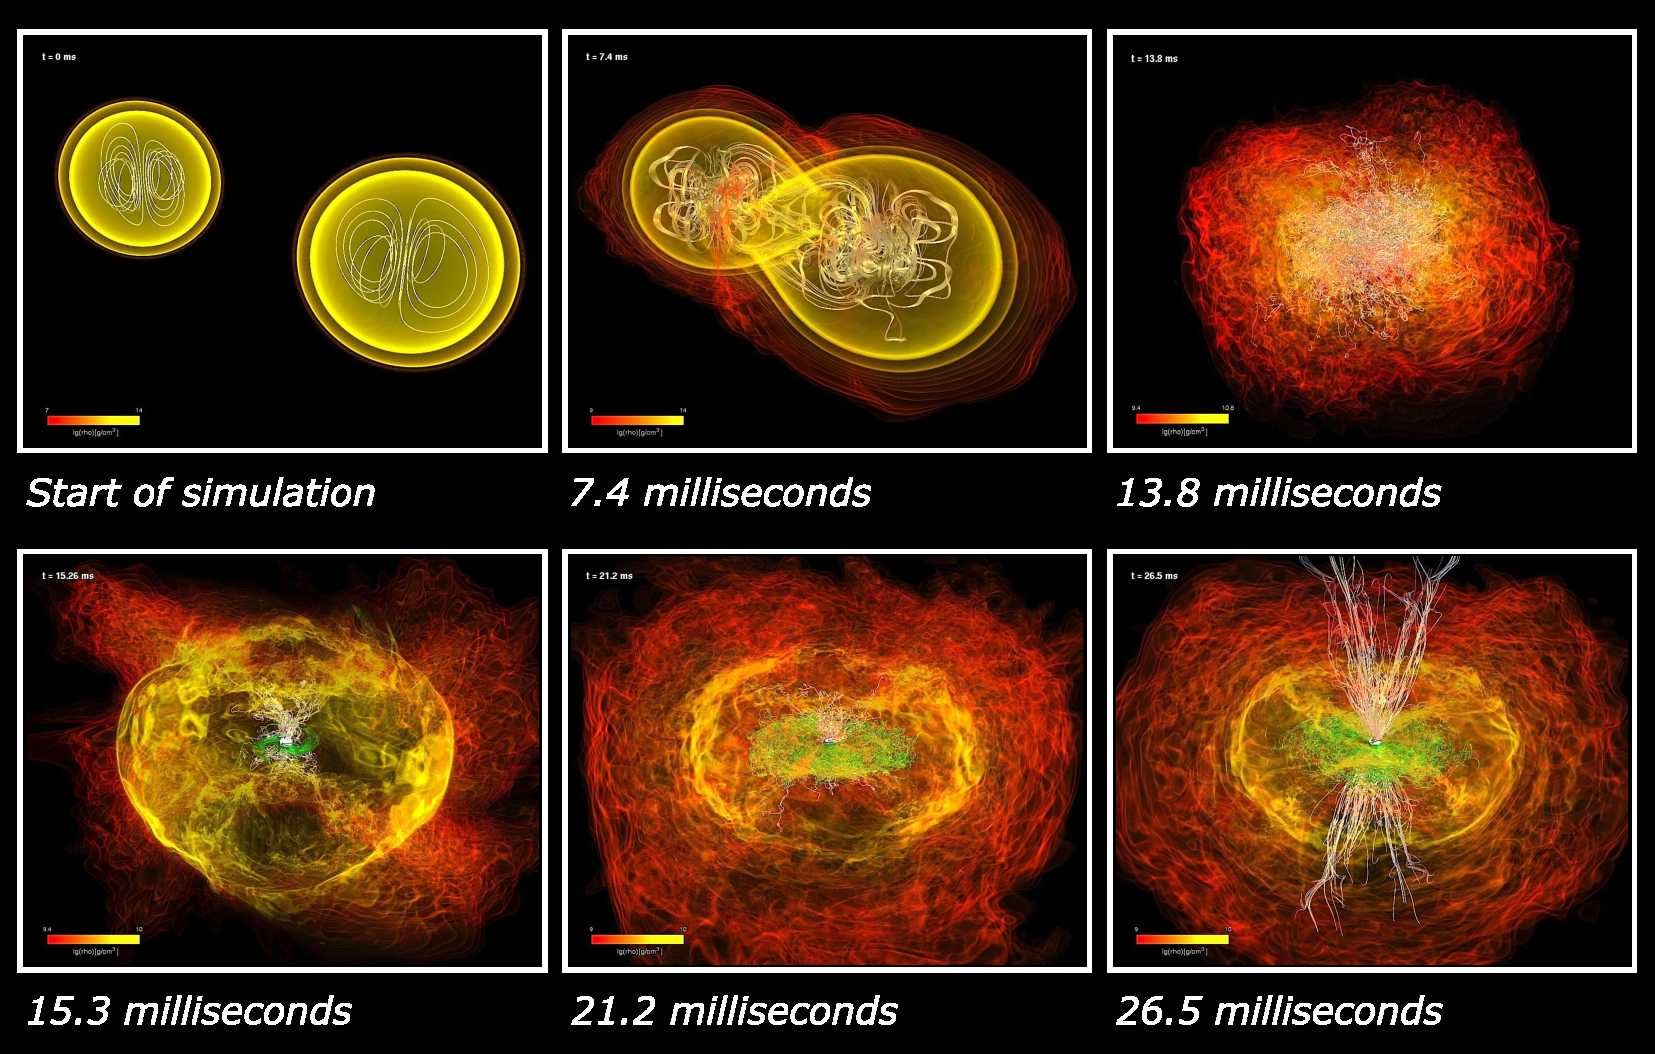
\includegraphics[width=0.88\linewidth,height=0.48\textheight,keepaspectratio]{../figs/pdf/en/fig-08-07.pdf}

% DOCX paragraph 1331
\caption{\emph{Distintas fases de una simulación numérica de la fusión de dos estrellas de neutrones magnetizadas. © M. Koppitz/C. Reisswig/LR.}}\label{fig:08-07}
\end{figure}

% DOCX paragraph 1333
Las simulaciones, que estaban a la vanguardia cuando se realizaron hace una década, empleaban varias simplificaciones y no carecían de limitaciones. Por ejemplo, aunque la geometría del campo magnético es correcta, las velocidades del plasma a lo largo del chorro son mucho menores que las medidas en los brotes cortos\index{brotes de rayos gamma!cortos} de rayos gamma. Sin embargo, su mayor mérito fue mostrar \emph{ab initio}, es decir, a partir de primeros principios, ya en 2011, que la presencia de un campo magnético es esencial para generar un chorro en la fusión de un sistema binario de estrellas de neutrones. En otras palabras, mediante la solución conjunta de las ecuaciones de Einstein y las de la magnetohidrodinámica\index{relativista!magnetohidrodinámica} relativista, estas simulaciones nos enseñaron que es posible reproducir la fenomenología observada en los brotes cortos de rayos gamma, al menos en términos de escalas temporales y liberación de energía, tras la colisión de dos estrellas de neutrones magnetizadas. Por desgracia, diez años después aún estamos lejos de simular de forma realista un brote corto de rayos gamma. Sin embargo, las simulaciones más modernas muestran cada vez con mayor claridad que los sistemas binarios de estrellas de neutrones magnetizadas son la vía más prometedora para comprender cómo puede producirse un chorro que se mueva hacia nosotros a velocidades relativistas, señalando uno de los sucesos más catastróficos del universo.

% DOCX paragraph 1334
En las horas y días posteriores a las primeras observaciones de GRB 170817A\index{GRB 170817A}, la señal electromagnética, que al principio estaba, obviamente, en la banda de los rayos gamma, siguió observándose a otras frecuencias gradualmente más bajas: pasó a los rayos X\index{rayos X!radiación}, luego al visible y, finalmente, al infrarrojo. Actualmente, después de varios cientos de días, todavía es posible detectar una emisión de GRB 170817A en la banda de radio. Esta señal se llama «\emph{resplandor residual\index{resplandor residual}}», o \emph{afterglow}, y se produce porque la fuente emisora se expande y se enfría a medida que se aleja del lugar de la fusión. Así, la emisión disminuye en intensidad y su máximo se desplaza hacia longitudes de onda cada vez mayores. No es muy distinto de lo que ocurre con los fuegos artificiales, cuando el brillo de la explosión se atenúa y desaparece al expandirse y enfriarse la nube de gas caliente.

% DOCX paragraph 1337
\section{Una explosión que vale su peso en oro}\label{sec:08-gold}

% DOCX paragraph 1339
Además del resplandor residual\index{resplandor residual}, la emisión de los brotes cortos\index{brotes de rayos gamma!cortos} de rayos gamma puede ir acompañada de una señal en las bandas ultravioleta y óptica de origen decididamente diferente: la desintegración radiactiva del material expulsado durante la fusión. De hecho, una característica muy robusta de la fusión de un sistema binario de estrellas de neutrones es que parte de la materia que inicialmente constituía las dos estrellas se expulsa a grandes distancias o, en una jerga más técnica, «se pierde en el infinito espacial». La razón es que parte de la materia de la colisión tiene mucha energía, con velocidades superiores a la velocidad de escape del campo gravitatorio del sistema. Las simulaciones aún no son lo bastante precisas para estimar cuánta masa se expulsa; depende de una serie de factores relacionados con las propiedades del sistema binario. No obstante, está bastante claro que oscila entre una décima de un por ciento y unos pocos por ciento de una masa solar. Dicho de otro modo, solo una fracción muy pequeña de la masa total del sistema se pierde realmente en el infinito, pero, como veremos, esa materia tiene una importancia enorme.

% DOCX paragraph 1340
Si parece bastante obvio que una parte de la materia del sistema binario pueda ser expulsada, lo que debería ocurrir con ella ya no lo es tanto. La primera predicción al respecto la hicieron en 1998 los astrónomos Li-Xin Li y Bohdan Paczyński\index{Paczyński, Bohdan}.\textsuperscript{\hyperlink{note:08-14}{14}} Con un modelo simplificado, Li y Paczyński razonaron que esa materia, rica en neutrones, es decir, compuesta por núcleos con muchos neutrones, pues originalmente formaba parte de estrellas de neutrones, podía experimentar desintegración radiactiva. Como resultado, generaría una emisión electromagnética, ya que, en términos generales, la materia radiactiva emite luz cuando se desintegra en elementos más ligeros, primero en el ultravioleta y, con el tiempo, en el visible y el infrarrojo. Esta señal electromagnética, de génesis muy distinta a la del resplandor residual\index{resplandor residual}, recibió el nombre de \emph{kilonova\index{kilonova}}, pues se estimaba que era unas 1000 veces, un kilo, más luminosa que la emitida por una \emph{nova\index{nova}}.\textsuperscript{\hyperlink{note:08-15}{15}} Y ocurrió algo sorprendente: se observó una señal de kilonova en GRB 170817A\index{GRB 170817A}, al registrarse una débil señal de desintegración unas 24 horas después de la primera emisión en rayos gamma. Al principio, la señal apareció con una emisión predominante en las longitudes de onda del azul\index{kilonova!azul}, de ahí el nombre de \emph{kilonova azul}, pero luego fue apagándose hacia longitudes de onda mayores, centradas en el rojo, una \emph{kilonova roja\index{kilonova!roja}}. Sin duda eran unos hermosos fuegos artificiales, pero también una sólida confirmación de la predicción de Li y Paczyński. La importancia de detectar una emisión de kilonova reside en que proporciona la prueba definitiva y convincente de que un brote corto de rayos gamma está intrínsecamente ligado a la fusión de estrellas de neutrones. Solo las estrellas de neutrones en un sistema de objetos compactos en fusión pueden expulsar materia con el alto contenido en neutrones necesario para producir y alimentar la señal de kilonova.\index{Li, Li-Xin}\index{brotes de rayos gamma!cortos}

% DOCX paragraph 1341
Pero hay más. La débil señal luminosa de la kilonova no solo nos dice que una porción muy pequeña de las estrellas de neutrones puede desintegrarse radiactivamente. También demuestra que el proceso de fusión distribuye por el espacio interestelar materia que contiene núcleos pesados y ricos en neutrones. Así resuelve otro problema que durante años ha tenido en vilo a la astronomía.

% DOCX paragraph 1342
Pero vayamos paso a paso. Hemos visto que, a lo largo de su vida, las estrellas transforman los elementos ligeros en otros cada vez más pesados mediante una cadena que empieza en el hidrógeno, produce helio, carbono, nitrógeno, neón y alcanza el hierro\index{hierro} en las estrellas más masivas. Recordemos también que los «elementos pesados» son los que tienen una masa\index{atomico@atómico!masa} atómica\index{masa!atómica} mayor que la del hierro, que es 56. Como ejemplos tenemos el estroncio\index{estroncio}, con una masa atómica de 88, el cesio (133), el europio (152), el platino\index{platino} (195), el oro\index{oro} (197) y, por supuesto, el uranio (238). Las estrellas solo pueden generar elementos pesados en cantidades muy pequeñas, dado que la principal cadena de producción nuclear está impulsada por procesos de fusión que comienzan con el hidrógeno y terminan con el hierro. Además, cuando estos procesos se agotan y las estrellas alcanzan las últimas etapas de su evolución, todos esos elementos, «pesados» o «ligeros», quedan atrapados en su interior, sin posibilidad de «esparcirse» por el espacio interestelar. Esta sencilla consideración nos lleva a preguntas bastante complejas: «¿Cómo pudo formarse un planeta como el nuestro, compuesto por elementos muy pesados, como el platino y el uranio? ¿De dónde obtuvo sus elementos pesados?».

% DOCX paragraph 1343
Una respuesta a estas preguntas llegó a principios de los años sesenta, cuando se comprendió que las estrellas masivas, cuyos núcleos contienen elementos tan pesados como el hierro\index{hierro}, pueden explotar como supernova\index{supernova}s y distribuir así esos elementos por el espacio interestelar. Además, tanto durante la propia explosión de supernova como durante la posterior expansión del material expulsado pueden darse procesos de \emph{nucleosíntesis}, procesos nucleares que sintetizan elementos pesados a partir de las cenizas de la estrella que ha explotado. Estos estudios muestran, por tanto, que las explosiones de supernova y la nucleosíntesis que las acompaña pueden generar elementos pesados como los que hemos mencionado. De ahí se sigue que toda la materia presente en la Tierra, incluidos nosotros, pues en pequeñas cantidades contenemos hierro y elementos pesados, es resultado del trabajo de nucleosíntesis realizado durante millones de años dentro de las estrellas. En otras palabras, somos «hijos e hijas de las estrellas»; bueno, al menos desde el punto de vista de la física nuclear\ldots{}

% DOCX paragraph 1344
El problema de esta idea, que solo ha salido a la luz en los últimos veinte años, es que esta explicación, aunque plausible y parcialmente correcta, no basta para explicar la abundancia de los elementos más pesados medida en las estrellas de nuestro entorno. En particular, los cálculos de la cantidad de estos elementos producida en explosiones de supernova indican una abundancia muy inferior a la observada. En otras palabras, hay demasiado oro\index{oro} en el universo, más del que pueden producir las explosiones de supernova\ldots{}

% DOCX paragraph 1345
A mediados de los años setenta se sugirió por primera vez una solución a este problema, cuando todavía no se había manifestado por completo su gravedad. Se señaló que las explosiones de supernova no son los únicos procesos capaces de expulsar grandes cantidades de material rico en neutrones y producir elementos pesados: la fusión de un sistema binario que contenga al menos una estrella de neutrones es igual de eficaz en ese sentido.\textsuperscript{\hyperlink{note:08-16}{16}} Inspirándose en esta sugerencia, en los últimos años se han realizado numerosas simulaciones, que han mostrado con gran claridad que la fusión de un sistema binario de estrellas de neutrones resulta ideal desde este punto de vista. Esto se debe a que las temperaturas y densidades alcanzadas durante la fusión son tan altas, y la materia ya es tan rica en neutrones, que la nucleosíntesis de elementos pesados es muy eficiente. Y eso no es todo: la abundancia de elementos pesados producidos así concuerda bien con las observaciones y solo depende débilmente de las propiedades del sistema binario. En esencia, el nuevo paradigma desarrollado durante la última década es que los sistemas binarios de estrellas de neutrones podrían ser el «lugar de producción» óptimo de los elementos pesados del universo.

% DOCX paragraph 1346
Sin embargo, todas estas consideraciones eran solo predicciones teóricas, nada más que el resultado de complejas simulaciones numéricas. A efectos prácticos, carecían de pruebas observacionales. Por fortuna, ¡GW170817\index{GW170817} lo cambió todo! La observación de la señal de kilonova\index{kilonova} ha confirmado que los sistemas binarios de estrellas de neutrones expulsan cantidades considerables de materia al espacio interestelar y que ese material puede sintetizar elementos pesados, tal como predicen las simulaciones teóricas. La confirmación fue posible porque la luz observada en la señal de kilonova\index{kilonova} de GRB 170817A\index{GRB 170817A} mostraba rastros de estroncio\index{estroncio}, un elemento pesado esencial. Era una de las pruebas reveladoras que se habían buscado durante años, ¡y la demostración indiscutible de que en la fusión de estrellas de neutrones de GW170817 se producen elementos pesados!

% DOCX paragraph 1347
Para captar lo extraordinario de este resultado, basta considerar que la cantidad de elementos pesados producidos en la nucleosíntesis que acompañó a GW170817\index{GW170817} equivale a 16\,000 veces la masa de la Tierra. Más impresionante aún es que una buena fracción de esos elementos pesados corresponde a platino\index{platino} y oro\index{oro}. Se han producido unas diez «masas terrestres», es decir, diez veces la masa de la Tierra, de platino y oro. Así que, si alguien busca oro, no tiene más que viajar en dirección a GW170817 y encontrará más del que pueda llevarse a casa\ldots{} Estas consideraciones nos enseñan además otra cosa: somos, en efecto, «hijos de las estrellas», ¡pero también «hijos de las estrellas de neutrones»!

% DOCX paragraph 1348
Quiero concluir este \emph{tour de force} sobre las estrellas de neutrones binarias con una consideración general. Soy plenamente consciente de que la cantidad de información que he transmitido puede resultar abrumadora, incluso confusa. Sin embargo, puedo asegurar que estos sistemas me impresionan tanto como a los lectores, y llevo décadas trabajando en ellos. ¿Cómo no asombrarse al saber que, en solo unas horas, GW170817\index{GW170817} ha dado respuestas claras a preguntas abiertas durante décadas? Con GW170817 hemos recibido confirmación de que las estrellas de neutrones en fusión son excelentes fuentes de ondas gravitatorias y emiten luz en forma de brotes cortos\index{brotes de rayos gamma!cortos} de rayos gamma. Además, expulsan unos pocos por ciento de una masa solar de materia especialmente rica en neutrones. Esa materia se reparte por el medio interestelar y produce la mayoría de los elementos pesados presentes en el universo, uno de los cuales, el oro, parece gustarnos especialmente a los humanos.

% DOCX paragraph 1349
Por todas estas razones, la fusión de un sistema binario de estrellas de neutrones representa un espectáculo de fuegos artificiales de increíble belleza y una fantástica combinación de fenómenos físicos. Todos los aspectos fundamentales de la física moderna convergen en este proceso: enormes curvaturas del espaciotiempo, emisión de ondas gravitatorias, hidrodinámica\index{relativista!hidrodinámica} relativista y física del plasma, física nuclear y síntesis de elementos. Por eso me gusta decir que las estrellas de neutrones binarias son \emph{«el laboratorio más rico de Einstein»}.

